\documentclass[svgnames,smaller,table]{beamer}
\usepackage{multirow}

\usetheme{ufmg}
\setbeamercolor*{normal text}{fg=black}
% -----------------------------------------------------------------------------------------------------------------

\title[Defesa de tese]{Acoplamento neutrônico e termo-hidráulico usando os
  códigos milonga e OpenFOAM: uma abordagem com \textit{software} livre}
\author{Vitor Vasconcelos Araújo Silva}
\date{19 de dezembro de 2016}
%\data{\today}
%\orientador{Cláubia Pereira Bezerra Lima}
%\coorientador{André Augusto Campagnole dos Santos}
\institute{%
  Universidade Federal de Minas Gerais -- UFMG
  \par
  Departamento de Engenharia Nuclear
  \par
  Programa de Pós-Graduação em Ciências e Técnicas Nucleares}

\begin{document}

%-------------------------------------------------
\begin{frame}
\titlepage
\end{frame}

%-------------------------------------------------
\begin{frame}
  \frametitle{Sumário}
  \tableofcontents%[pausesections]
\end{frame}


\section{O que é isso?}
%-------------------------------------------------
\begin{frame}
  \frametitle{O que é isso?}
  \framesubtitle{Definições}
  \begin{itemize}
  \item \textbf{Neutrônica:} Estudo do transporte de nêutrons.
  \item \pause \textbf{Termo-hidráulica:} Estudo da transferência de calor e massa, processos fluido-mecânicos com transporte
    de energia e massa em sistemas nucleares \cite{Todreas2012}.
  \item \pause \textbf{Acoplamento (ou multifísica):} Análise de fenômenos físicos distintos de forma combinada \cite{Lethbridge2005}.
  \end{itemize}
  E por que acoplar?
  
\end{frame}

\subsection{Justificativa}
%-------------------------------------------------
\begin{frame}
  \frametitle{Justificativa}
%  \framesubtitle{}
  
\end{frame}

\subsection{Exemplo}
%-------------------------------------------------
\begin{frame}
  \frametitle{Exemplo}
  \framesubtitle{Exemplo1}
  
\end{frame}

\section{Percurso}
%-------------------------------------------------
\begin{frame}
  \frametitle{Percurso}
  \framesubtitle{O caminho é tortuoso...}
  \textbf{Inicialmente:} \textit{Desenvolvimento do Acoplamento
Neutrônico e Termo-hidráulico usando os códigos PARCS
e OpenFOAM: Aplicação à Segurança de Reatores} \cite{PARCS2006}

  \begin{itemize}
    \item Trabalho \cite{Silva2013} e registro de \textit{software} \cite{TrigaFuel2013}.
  \end{itemize}
   \textbf{Doutorado sanduíche:} Universidade Politécnica de Valência.
    Acoplamento com código da UPV, dessa vez aplicado a reatores
    de potência (PWR).
  \begin{itemize}
    \item Trabalho \cite{Silva2015}.
  \end{itemize}
  \textbf{Finalmente:} \textit{Acoplamento neutrônico termo-hidráulico usando
    os códigos milonga e OpenFOAM: uma abordagem com sotware livre}.
  \begin{itemize}
    \item Artigo (aceito).
  \end{itemize}
  \centering
  \pause \alert{Esta tese!}

\end{frame}

\subsection{Ferramentas}
%-------------------------------------------------
\begin{frame}
  \frametitle{Ferramentas}
  \framesubtitle{Neutrônica}
  
\end{frame}

%-------------------------------------------------
\section{Aplicação}
\begin{frame}
  \frametitle{Como provar o conceito?}
  \begin{itemize}
  \item Sistema acoplado funcional
  \item Malha idêntica
  \item Baseado em \textit{software} livre
  \end{itemize}
\end{frame}

%-------------------------------------------------
\subsection{Condições iniciais}
\begin{frame}
  \frametitle{Condições iniciais}
  \framesubtitle{Temperaturas médias iniciais}
  
    \centering
    Temperaturas médias iniciais de referência.
    \label{tab:temp-keff}
    \begin{tabular}{cccc}
      \multicolumn{1}{l}{}         & \multicolumn{3}{c}{Temperaturas [K]}                                                                        \\ \cline{2-4}
      \multicolumn{1}{c}{Potência [kW]} & \multicolumn{1}{c}{Refrigerante} & \multicolumn{1}{c}{Revestimento} & \multicolumn{1}{c}{Combustível}  \\ \hline
      1.98                      & 303,56                         & 327,20                         & 339,80                           \\ \hline
      3.97                      & 307,15                         & 354,54                         & 379,77                           \\ \hline
      7,93                      & 310,09                         & 375,42                         & 422,94                                         
    \end{tabular}
\end{frame}

%-------------------------------------------------
\begin{frame}
  \frametitle{Condições iniciais}
  \framesubtitle{Distribuição de potências iniciais}
  %  Fluxo [$\phi/phi_{avg}$].
%  \centering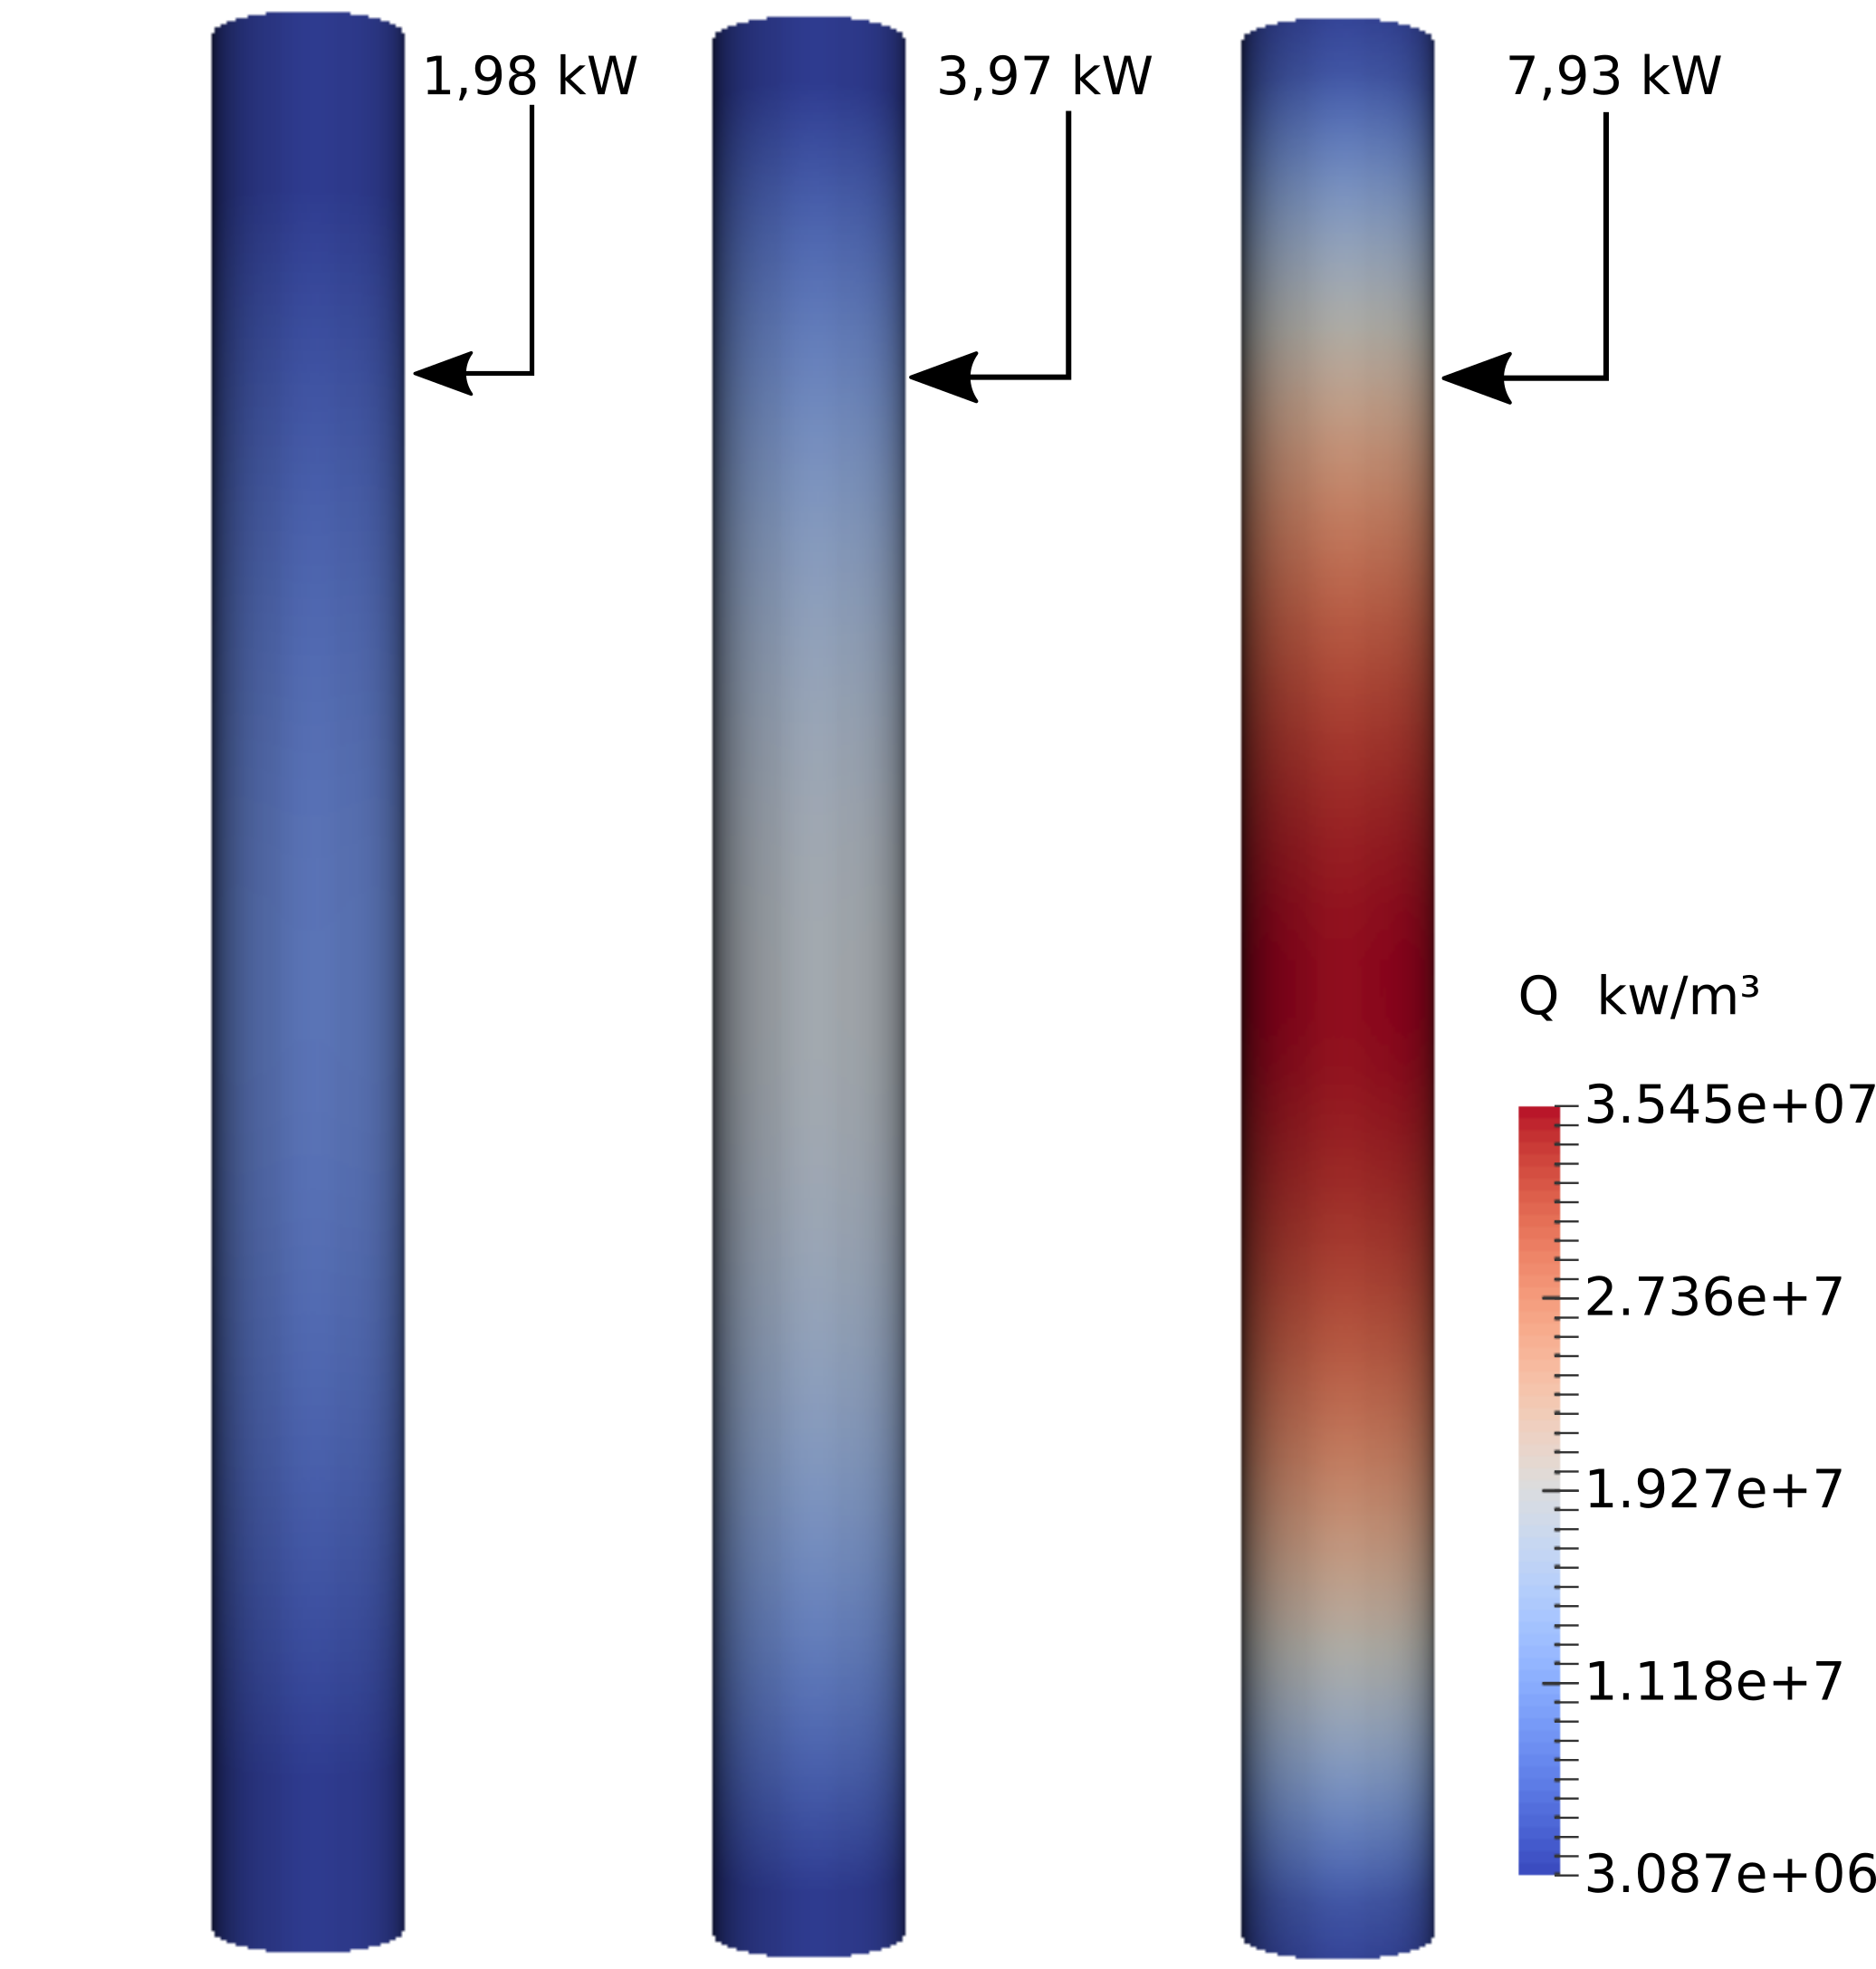
\includegraphics[width=\textwidth, height=7.0cm]{../figuras/Q_fuel_all_NC.png}
  \centering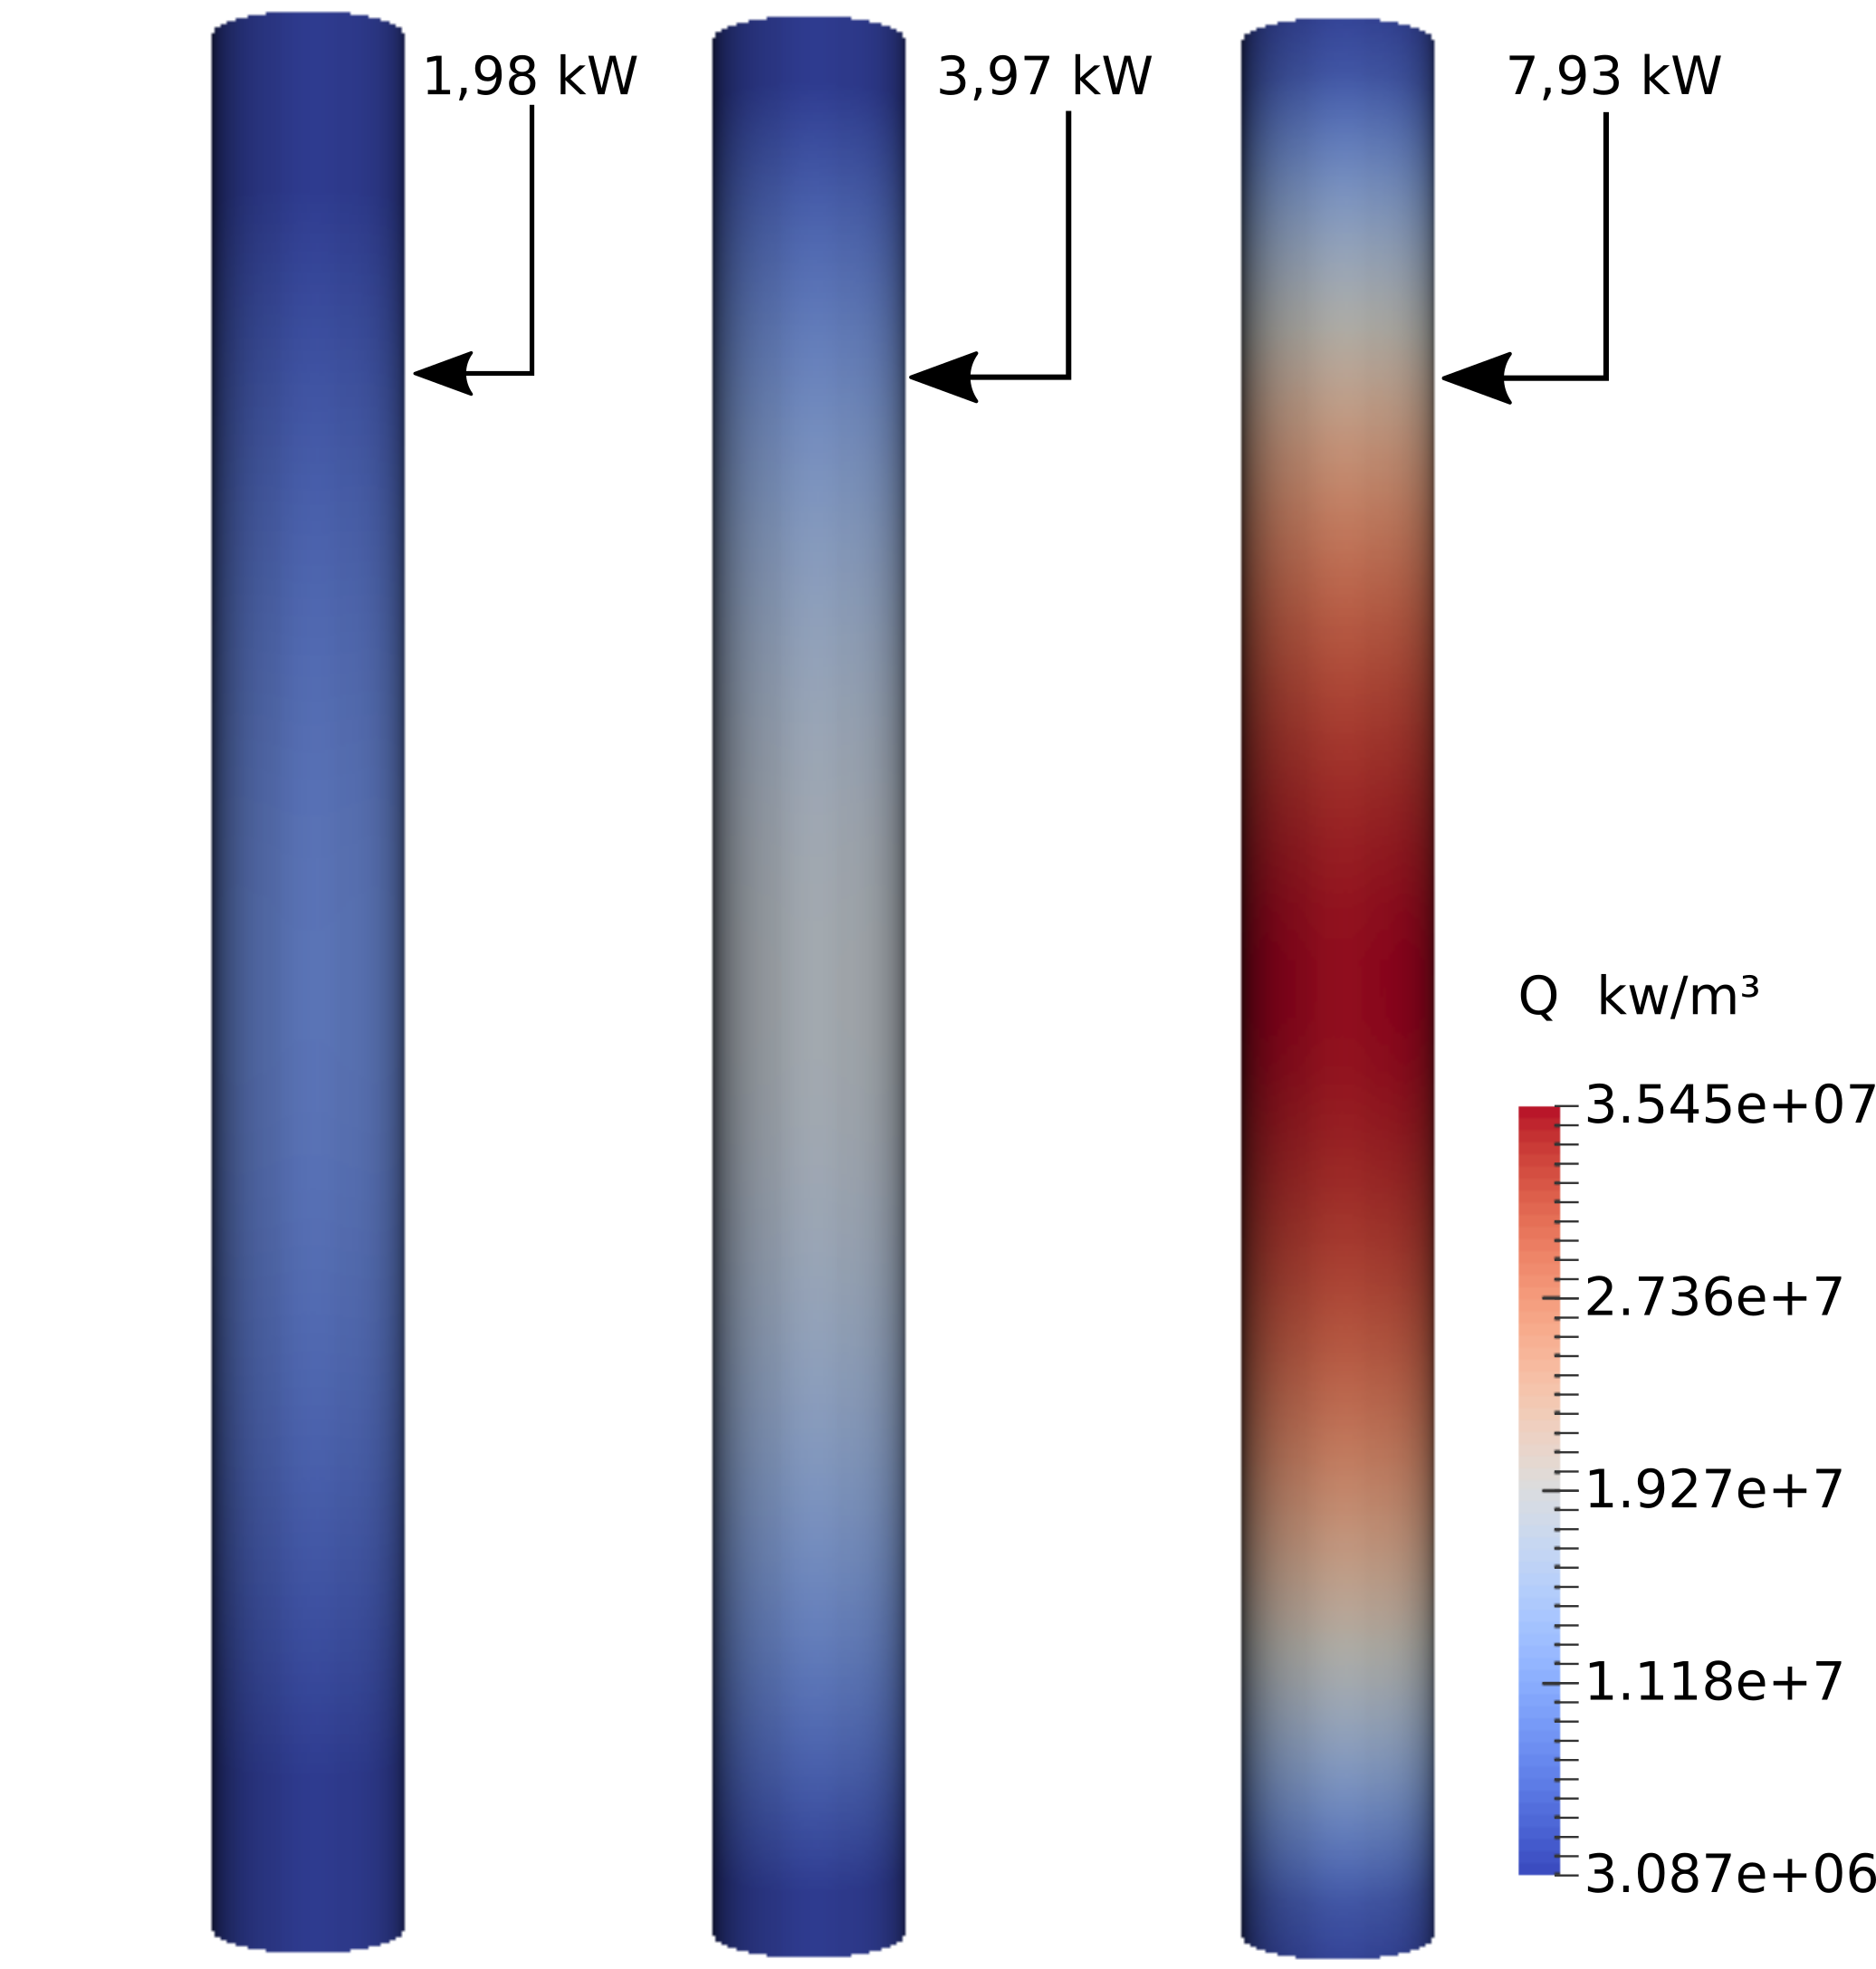
\includegraphics[scale=0.4]{../figuras/Q_fuel_all_NC.png}
\end{frame}

%-------------------------------------------------
\subsection{Gráficos}
\begin{frame}
  \frametitle{Resultados}
  \framesubtitle{Fluxo neutrônico: distribuição axial ($7,93 kW$)}
  %  Fluxo [$\phi/phi_{avg}$].
  \centering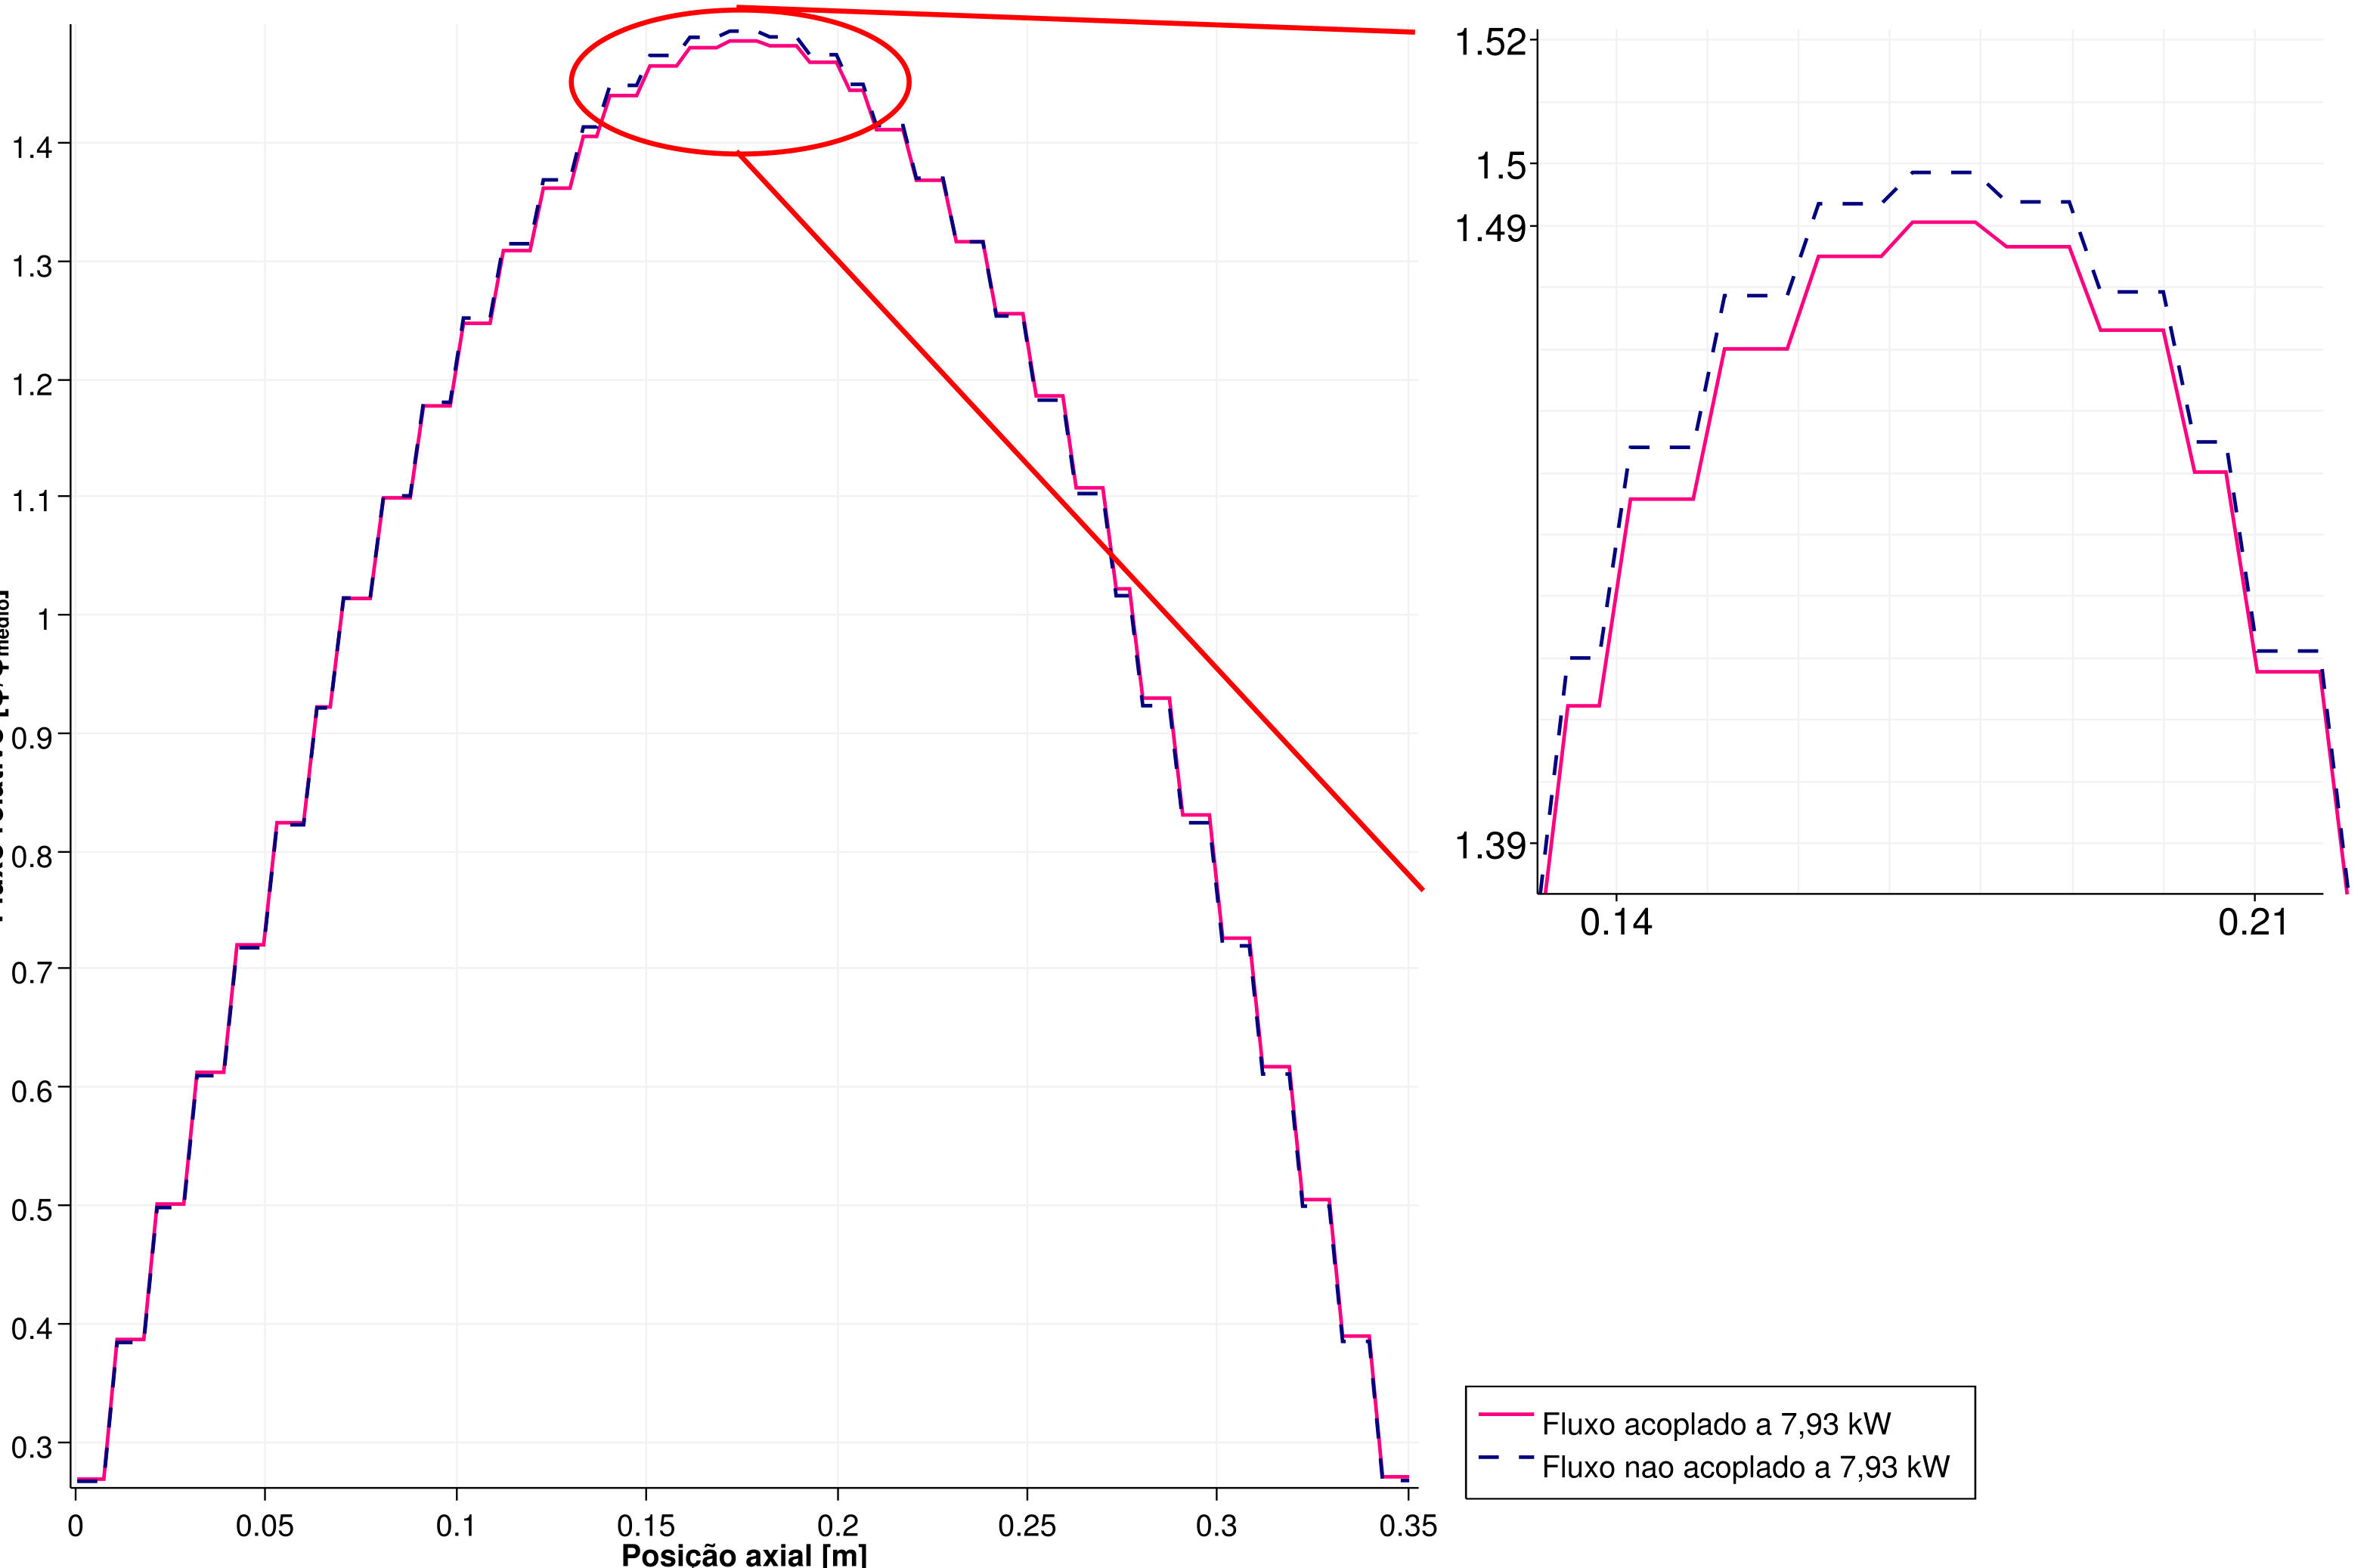
\includegraphics[width=\textwidth, height=7.0cm]{../figuras/Flux_rel_z_200_port_trabalhado.png}
  \label{fig:flux200z}
\end{frame}

%-------------------------------------------------
%\subsection{Gráficos}
\begin{frame}
  \frametitle{Resultados}
  \framesubtitle{Fluxo neutrônico: distribuição radial ($7,93 kW$)}
%  Fluxo [$\phi/phi_{avg}$].
  \centering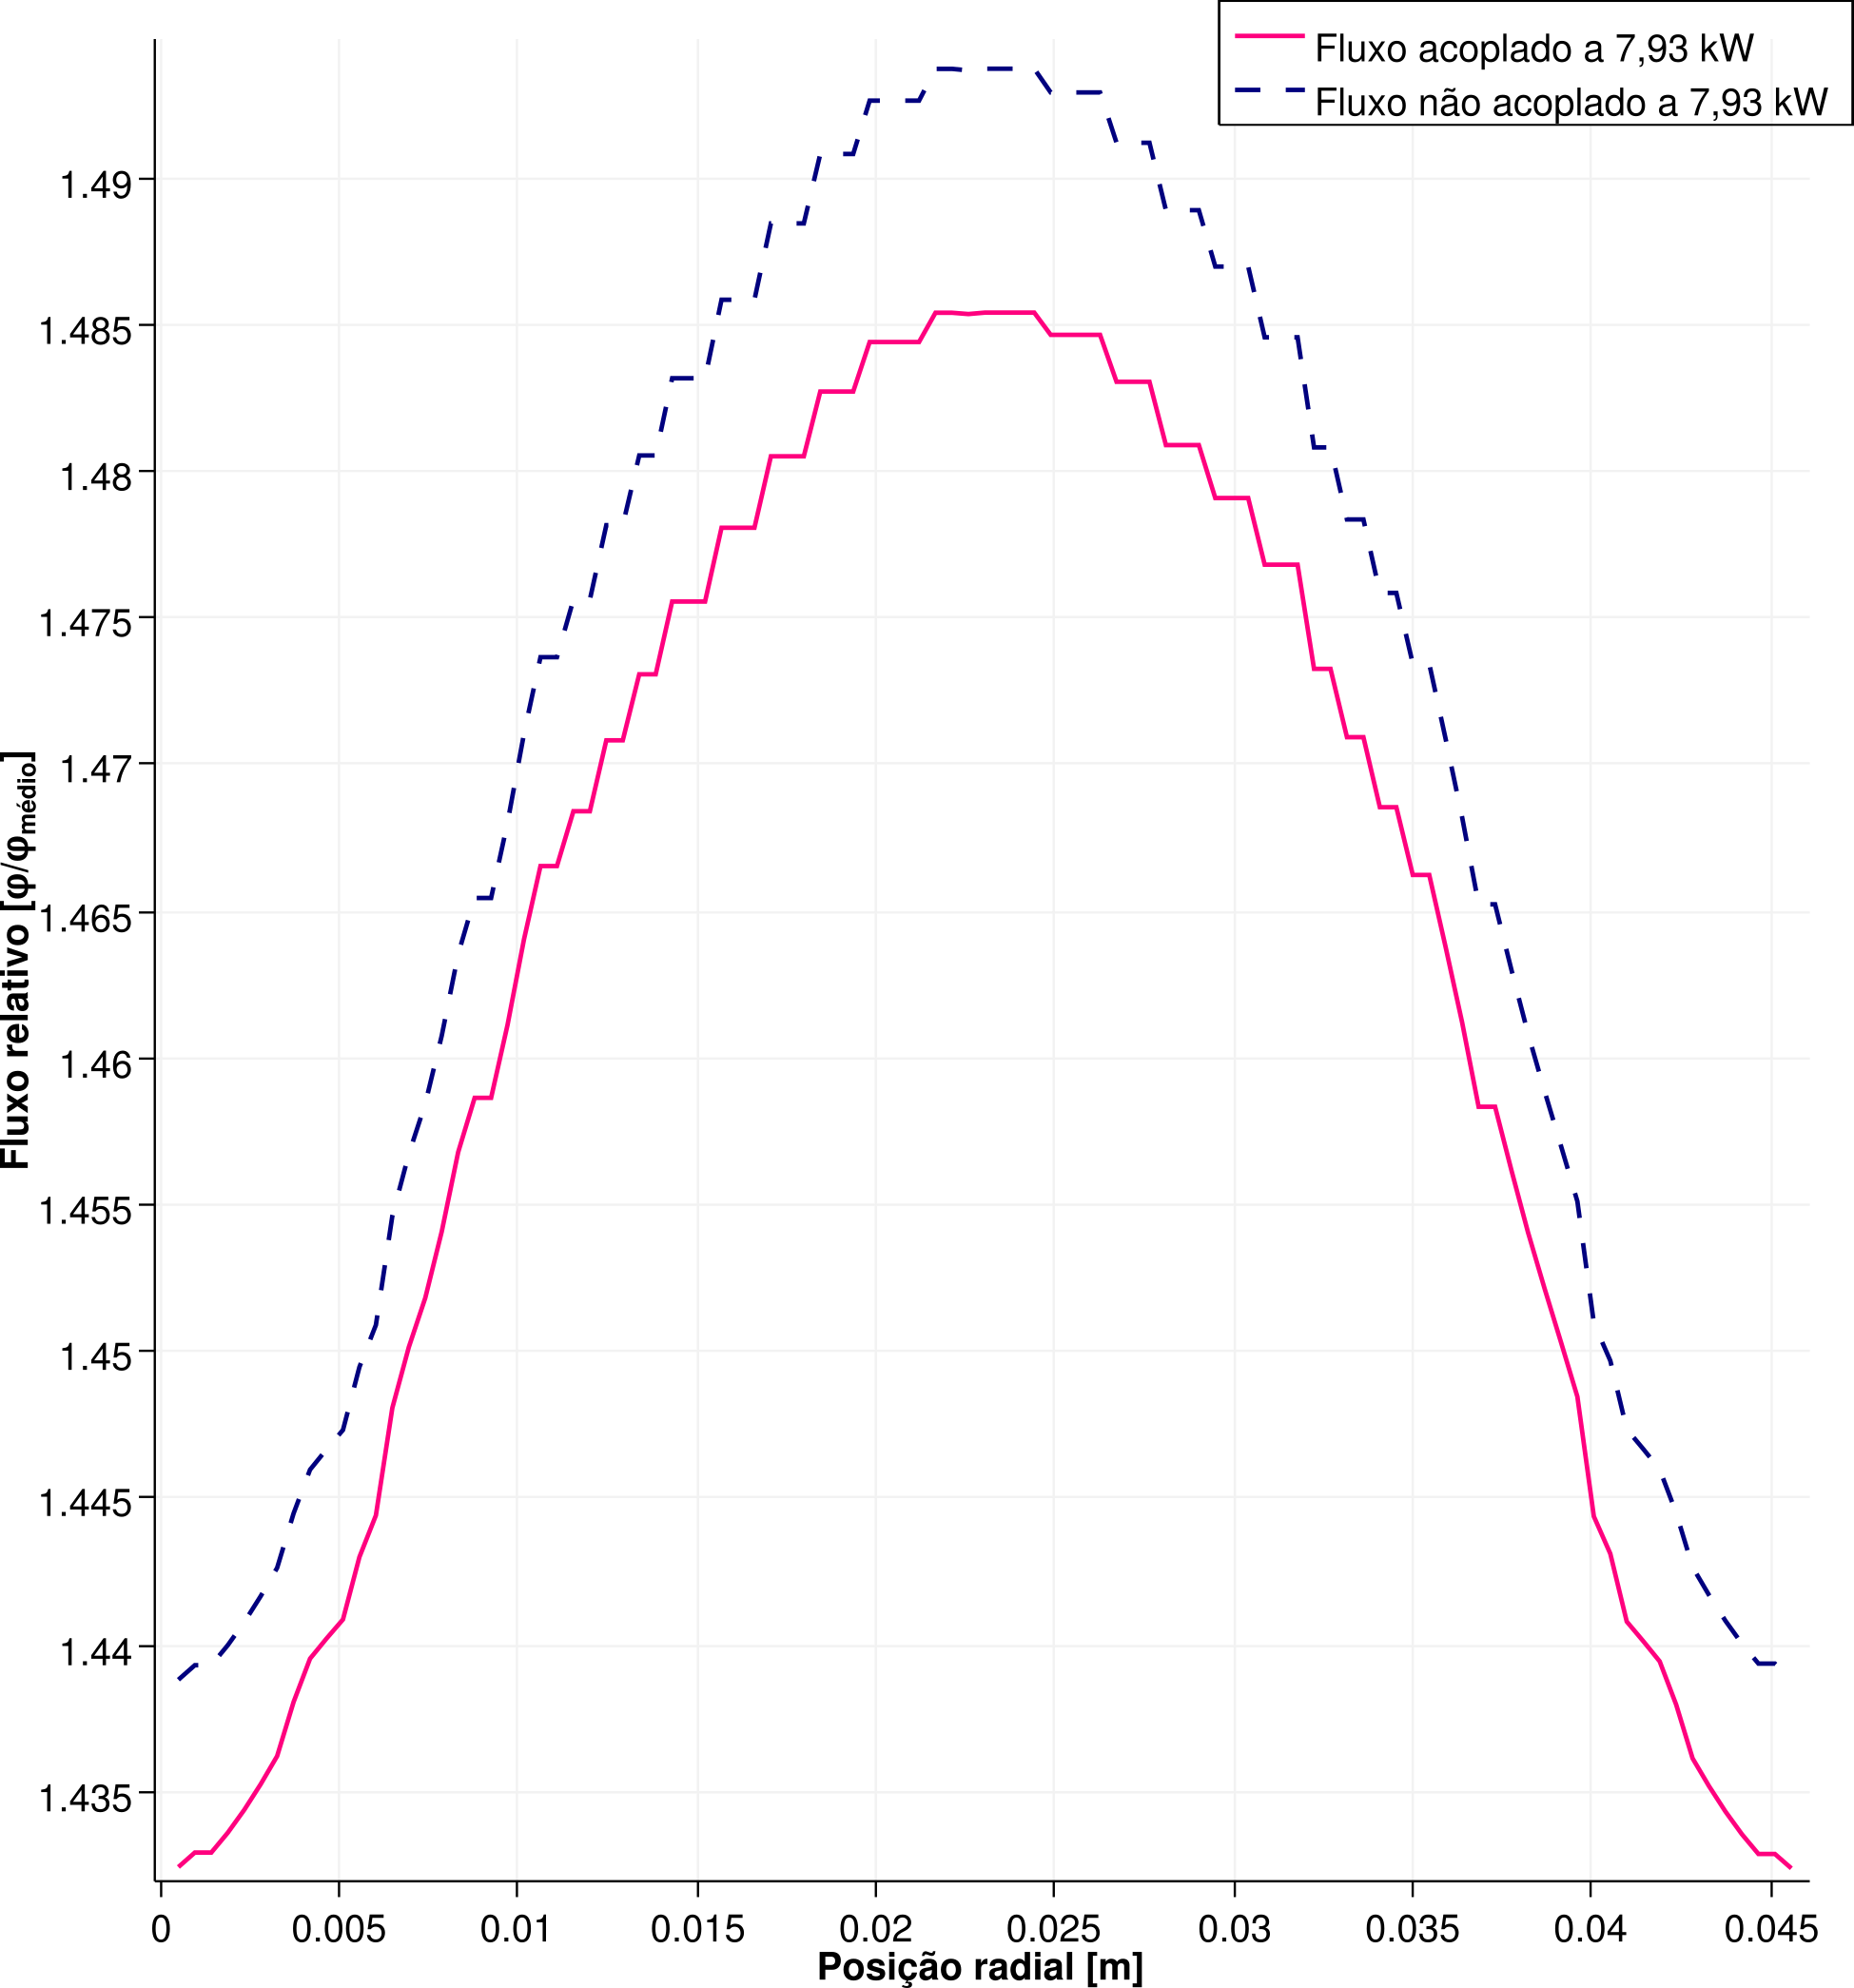
\includegraphics[width=\textwidth, height=7.0cm]{../figuras/Flux_rel_x_200_port.png}
  \label{fig:flux200x}
\end{frame}

%-------------------------------------------------
%\subsection{Gráficos}
\begin{frame}
  \frametitle{Resultados}
  \framesubtitle{Potência: distribuição axial}
%  Distribuição de potência [$kW/m^3$].
  \centering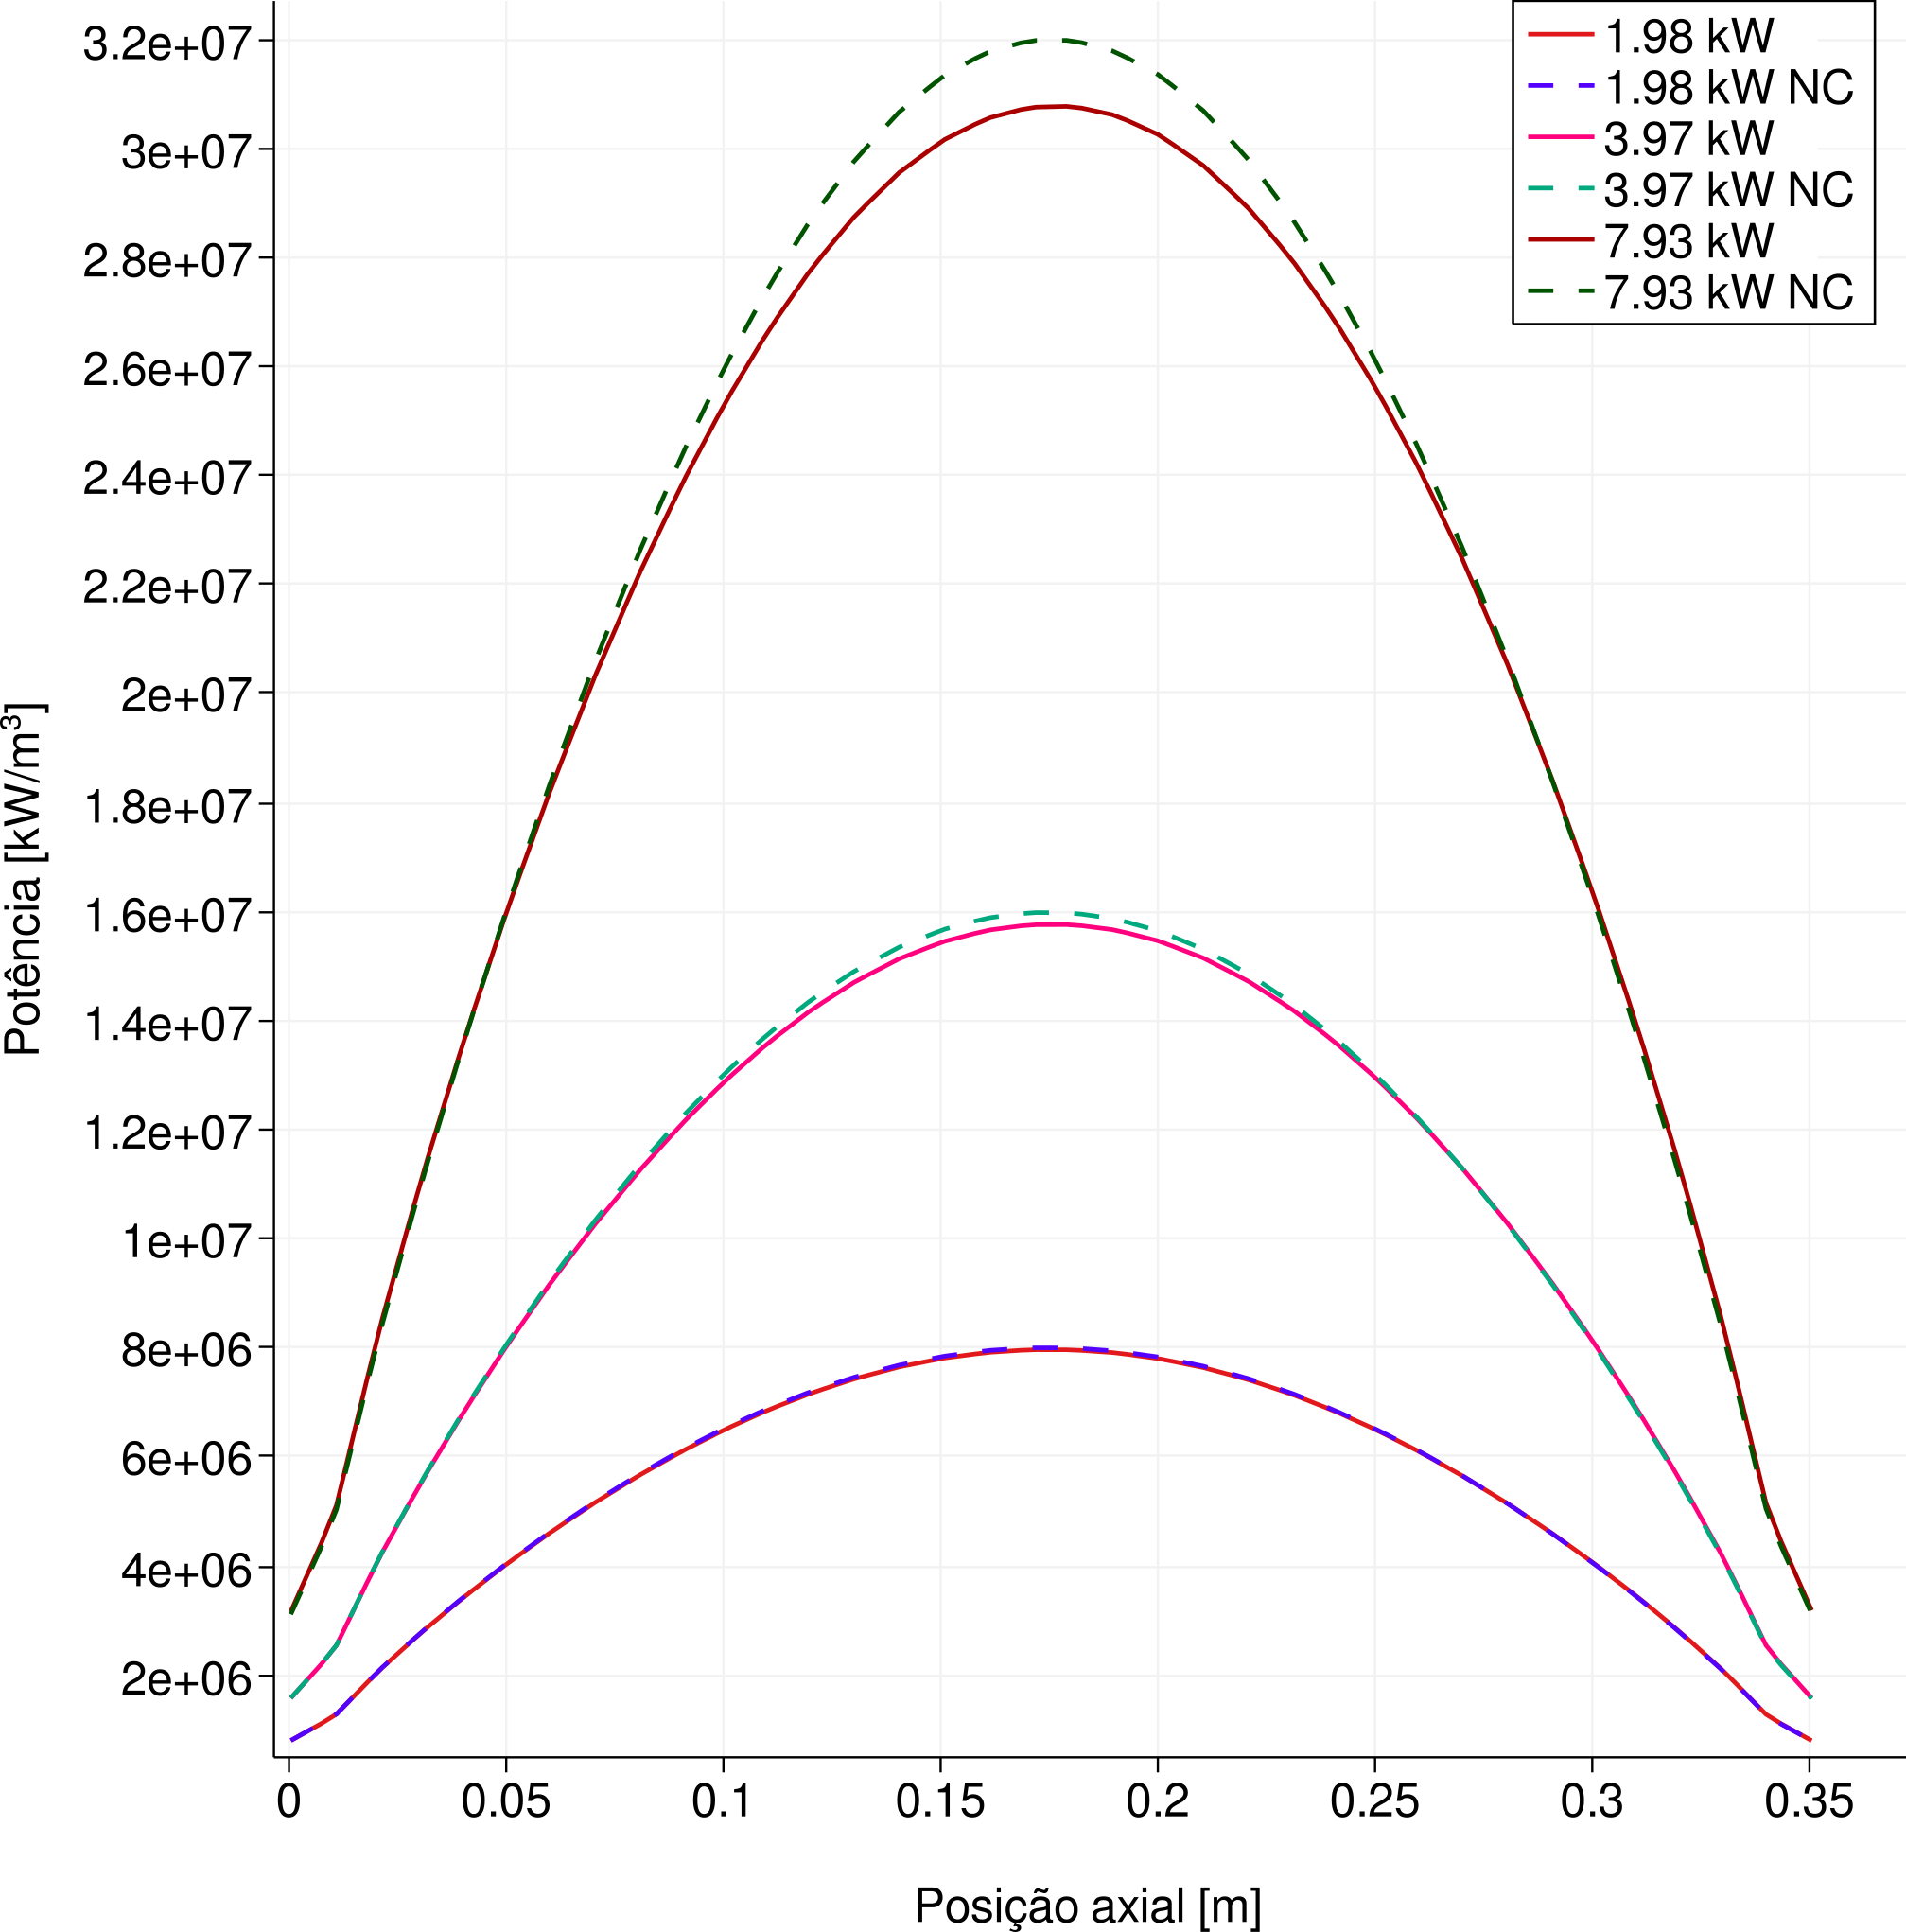
\includegraphics[width=\textwidth, height=7.0cm]{../figuras/Q_all_z_square_port.png}
  \label{fig:keff50}
\end{frame}

%-------------------------------------------------
%\subsection{Gráficos}
\begin{frame}
  \frametitle{Resultados}
  \framesubtitle{Potência: distribuição radial}
%  Distribuição de potência [$KW/m^3$].
  \centering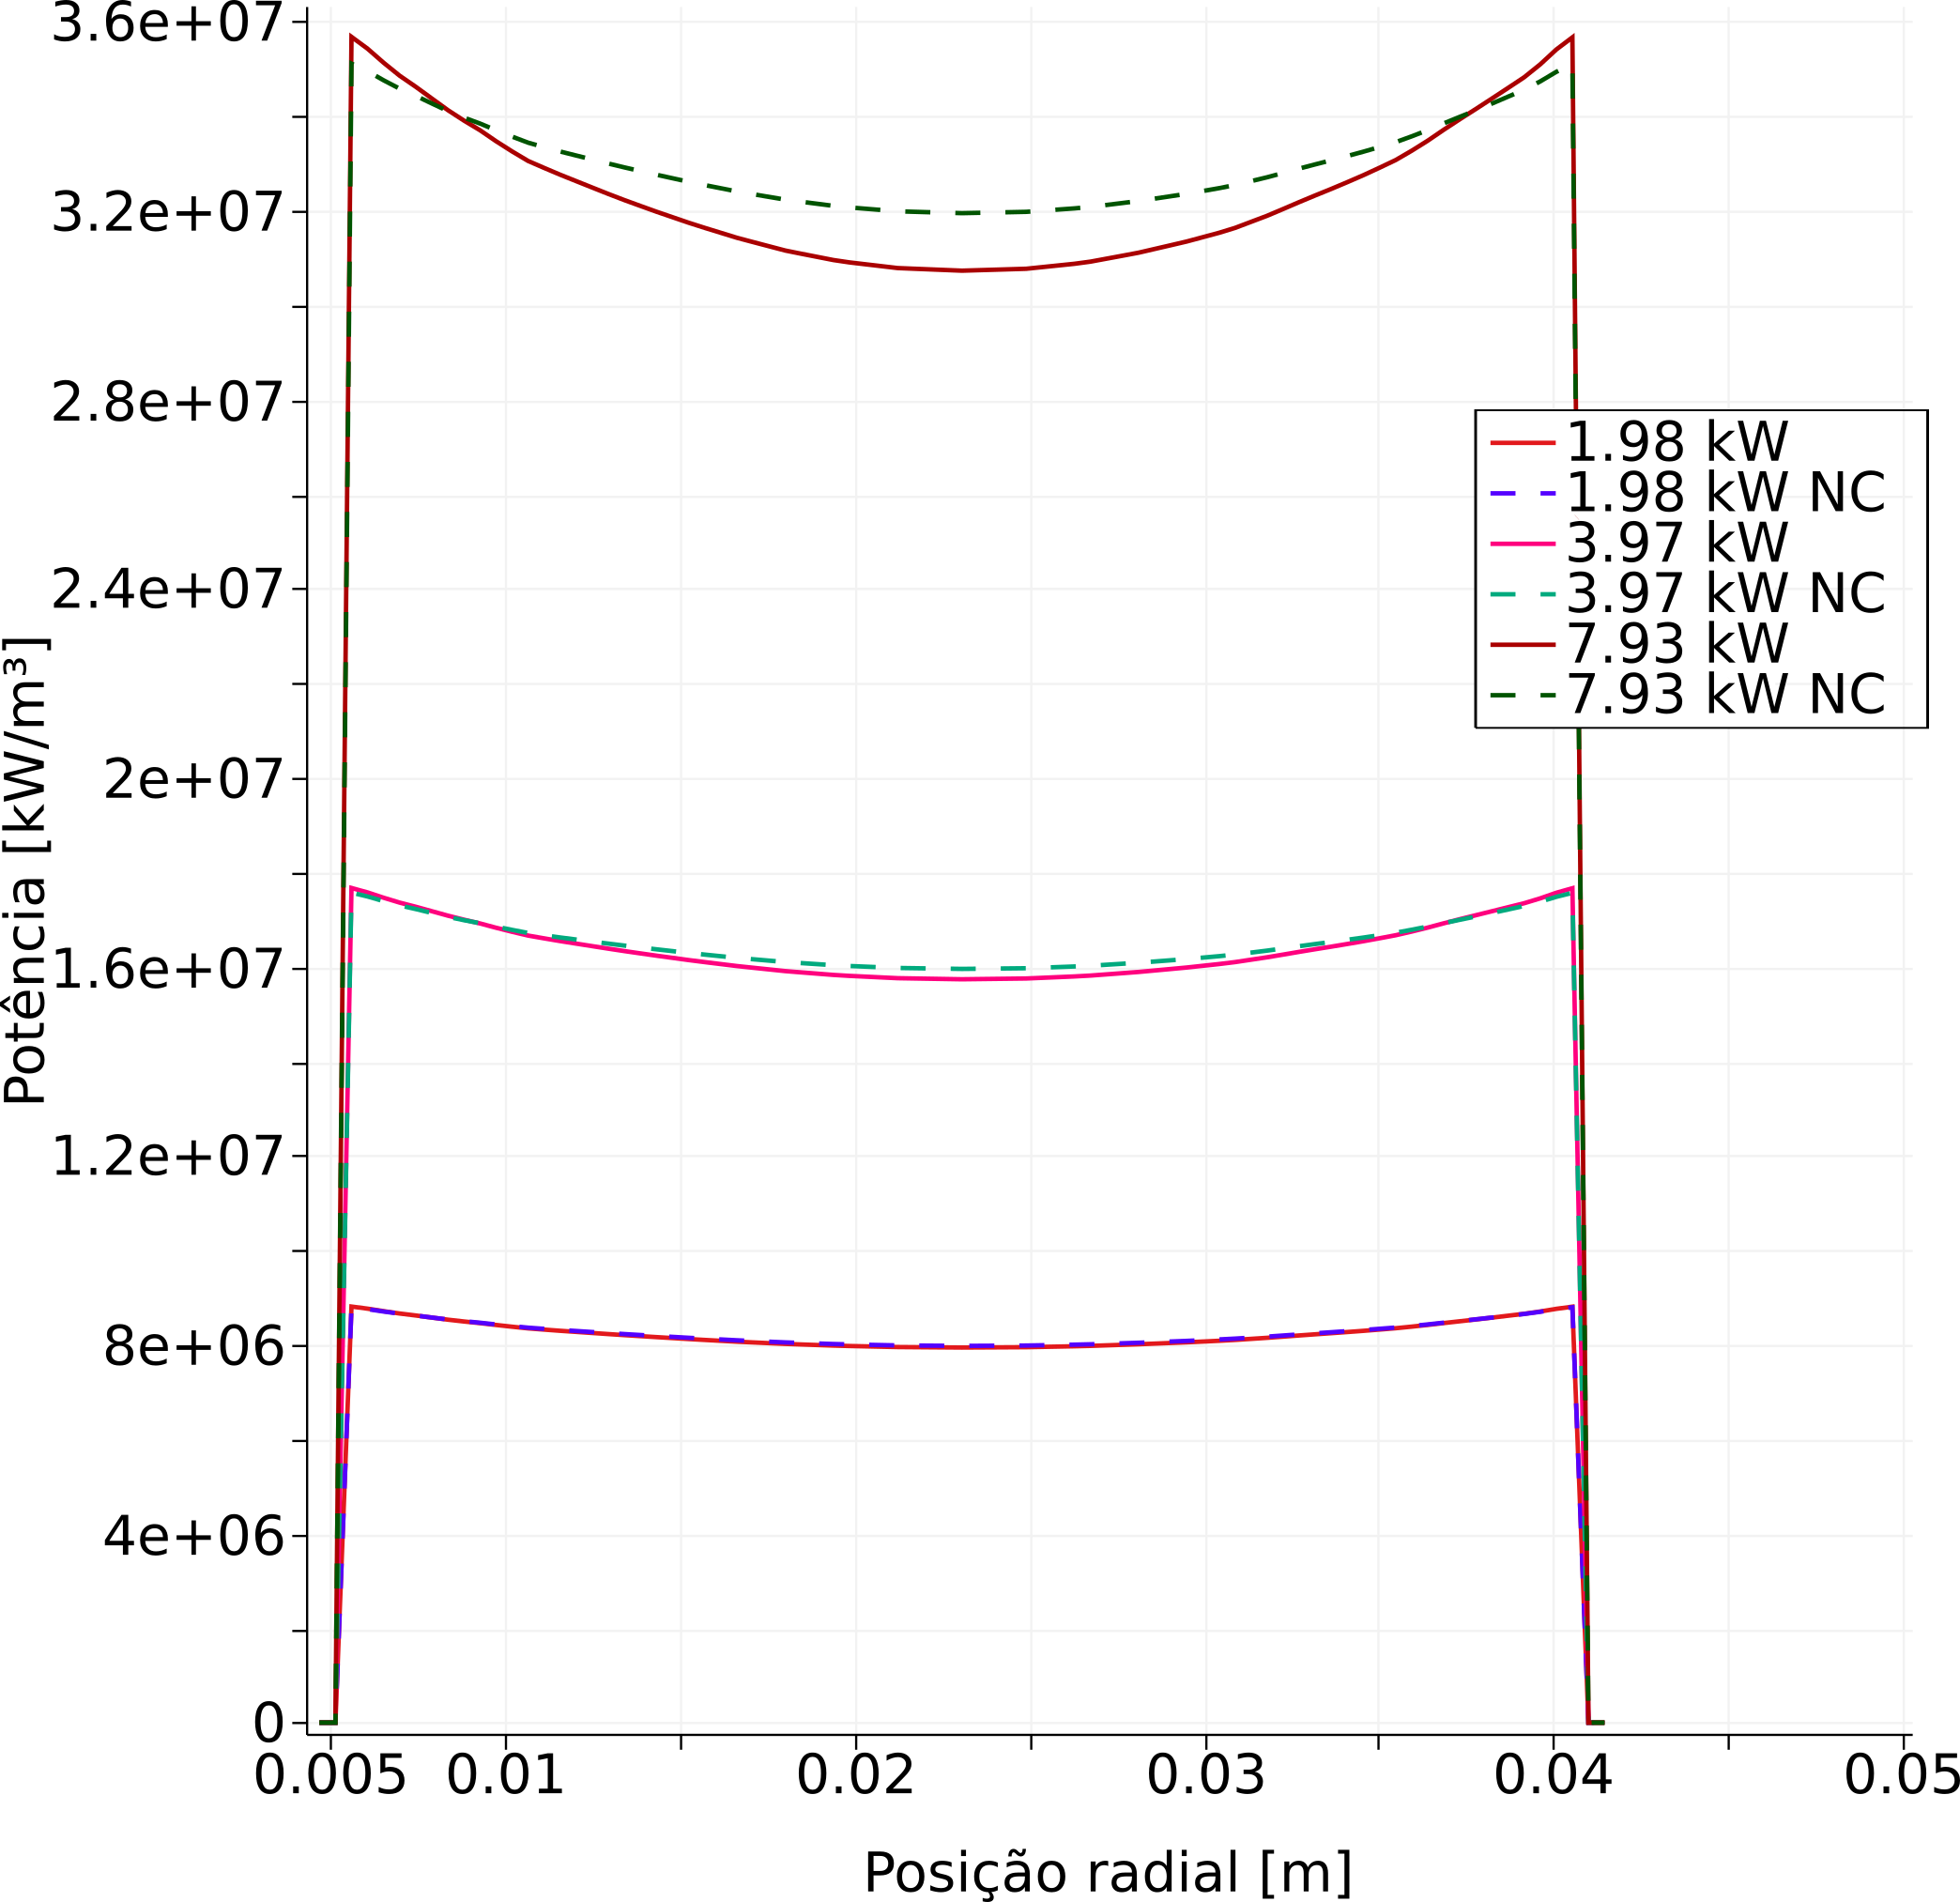
\includegraphics[width=\textwidth, height=7.0cm]{../figuras/Q_all_x_square_port.png}
  \label{fig:keff50}
\end{frame}

%-------------------------------------------------
%\subsection{Gráficos}
\begin{frame}
  \frametitle{Resultados}
  \framesubtitle{Temperatura: distribuição axial}
%  Distribuição de temperaturas [$K$].
  \centering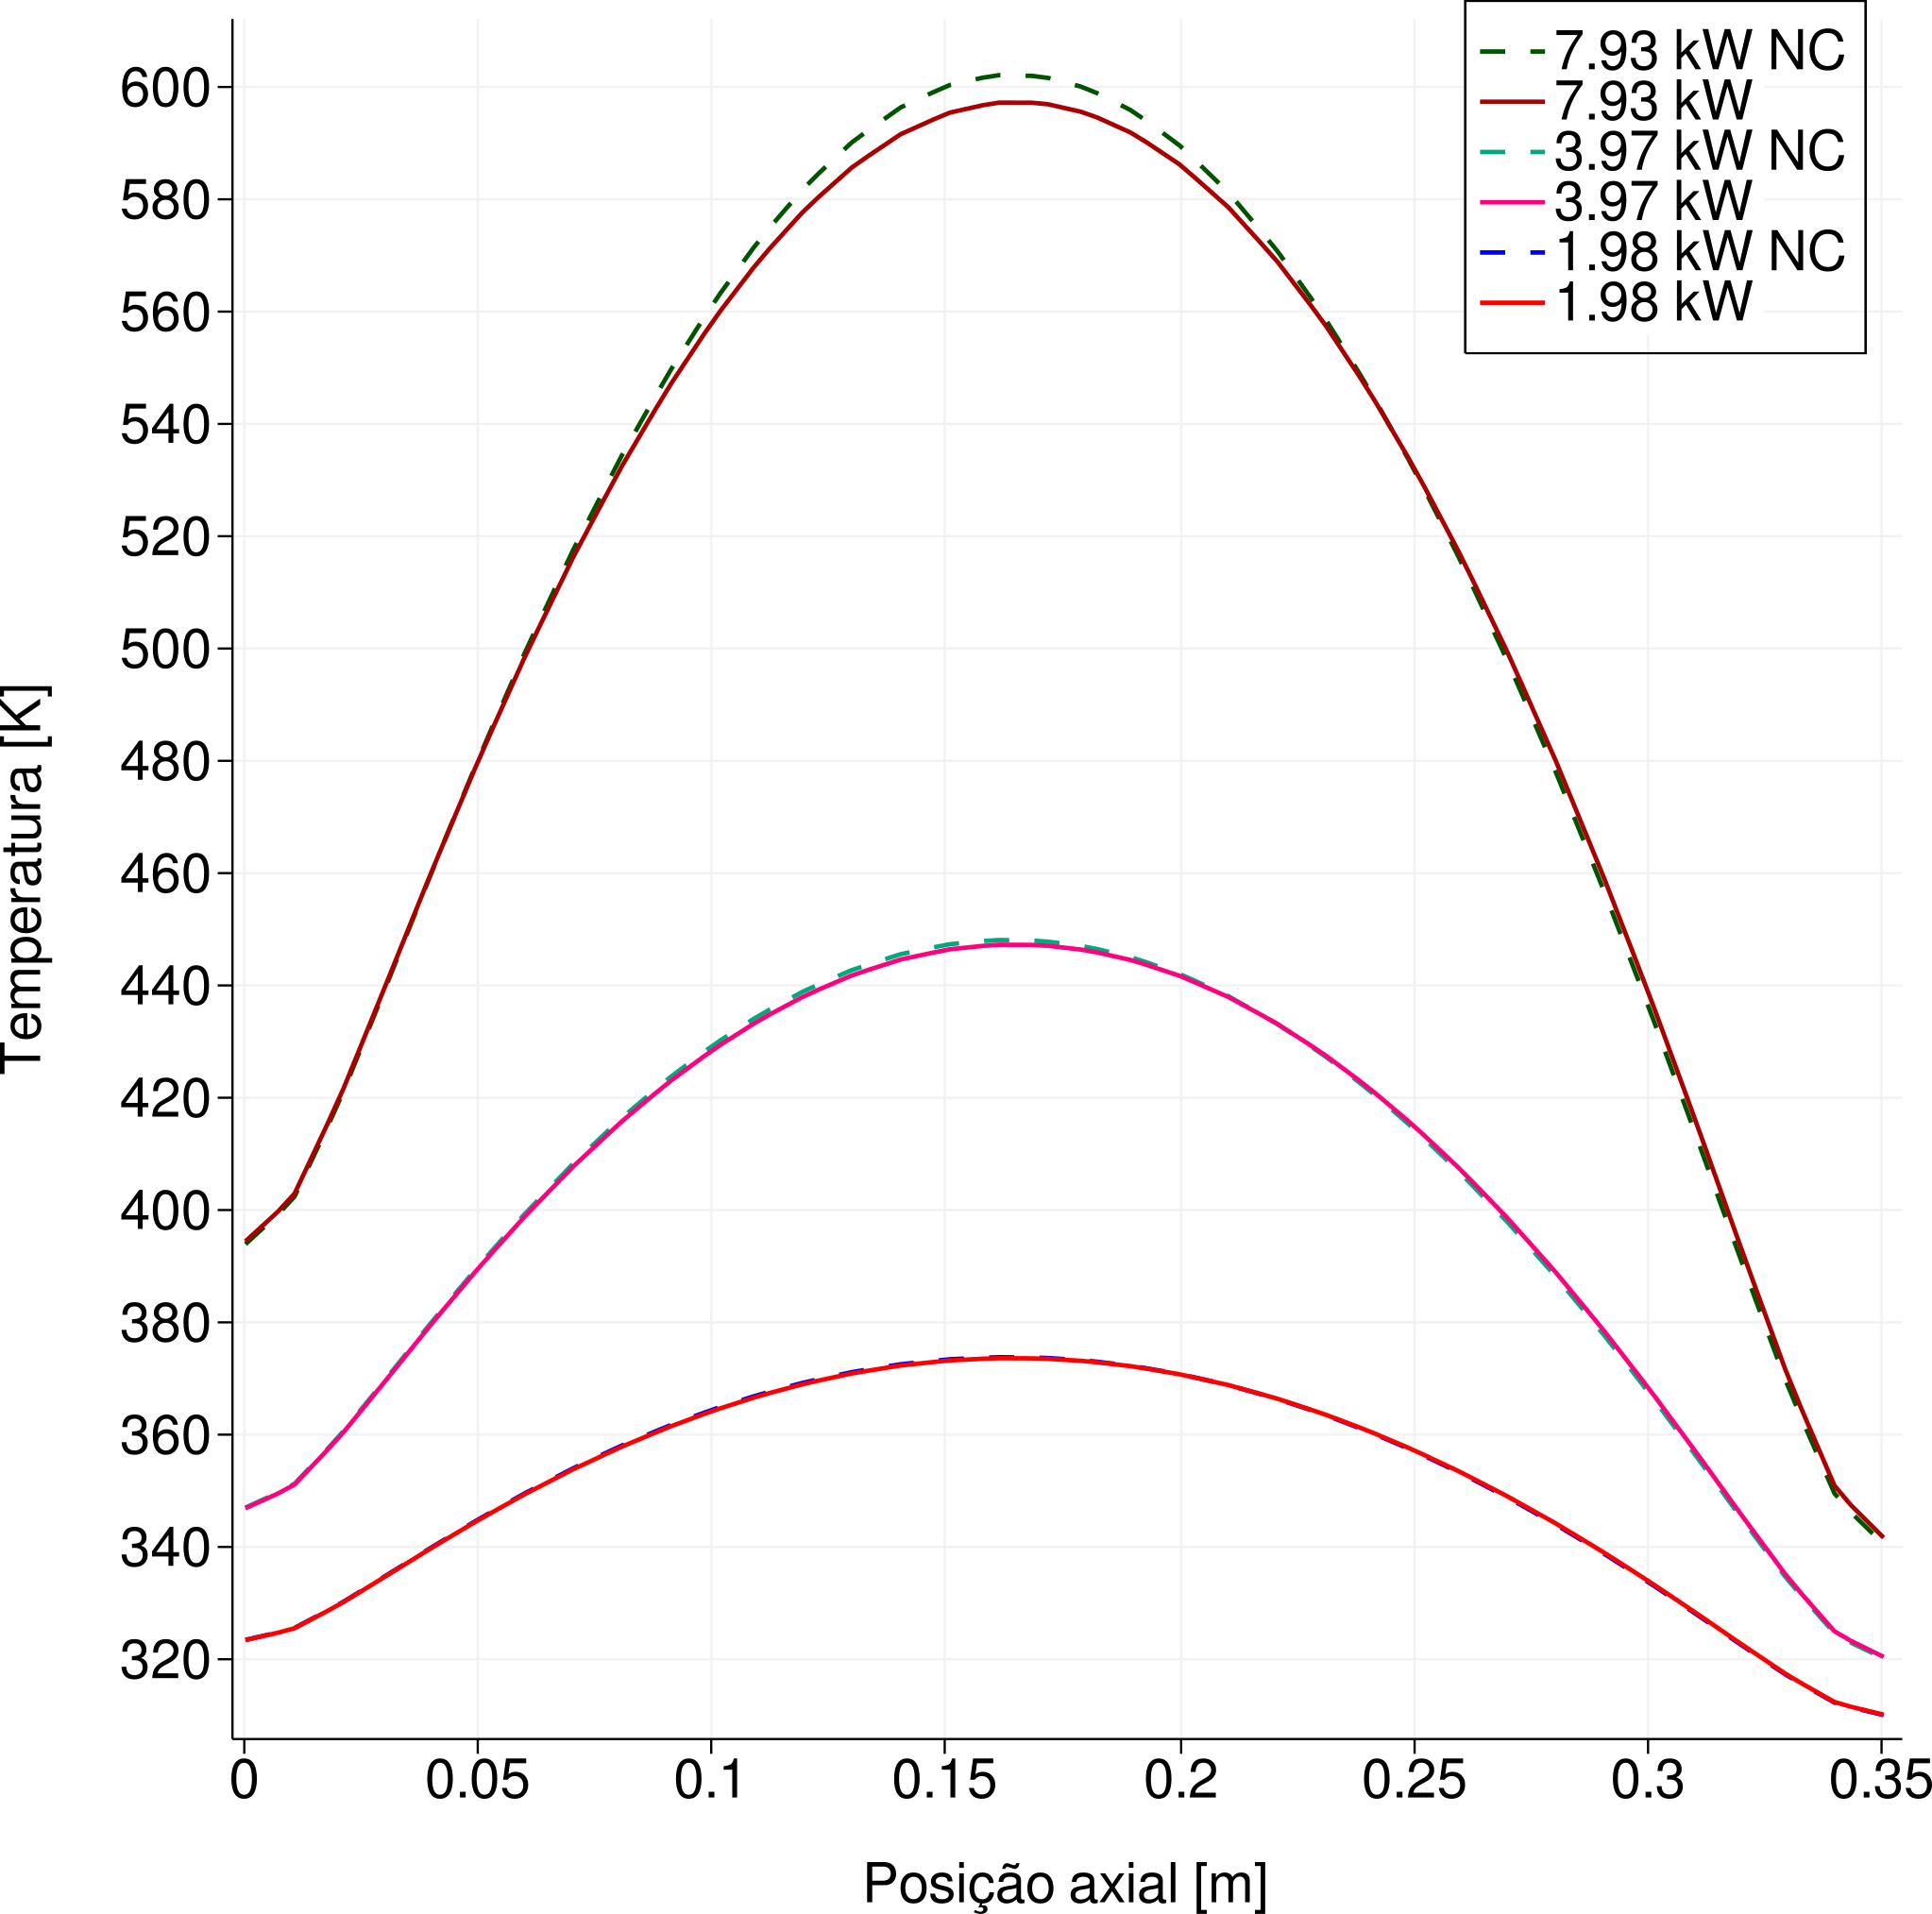
\includegraphics[width=\textwidth, height=7.0cm]{../figuras/T_z_all_square_port.png}
  \label{fig:keff50}
\end{frame}

%-------------------------------------------------
%\subsection{Gráficos}
\begin{frame}
  \frametitle{Resultados}
  \framesubtitle{Temperatura: distribuição radial}
%  Distribuição de temperaturas [$K$].
  \centering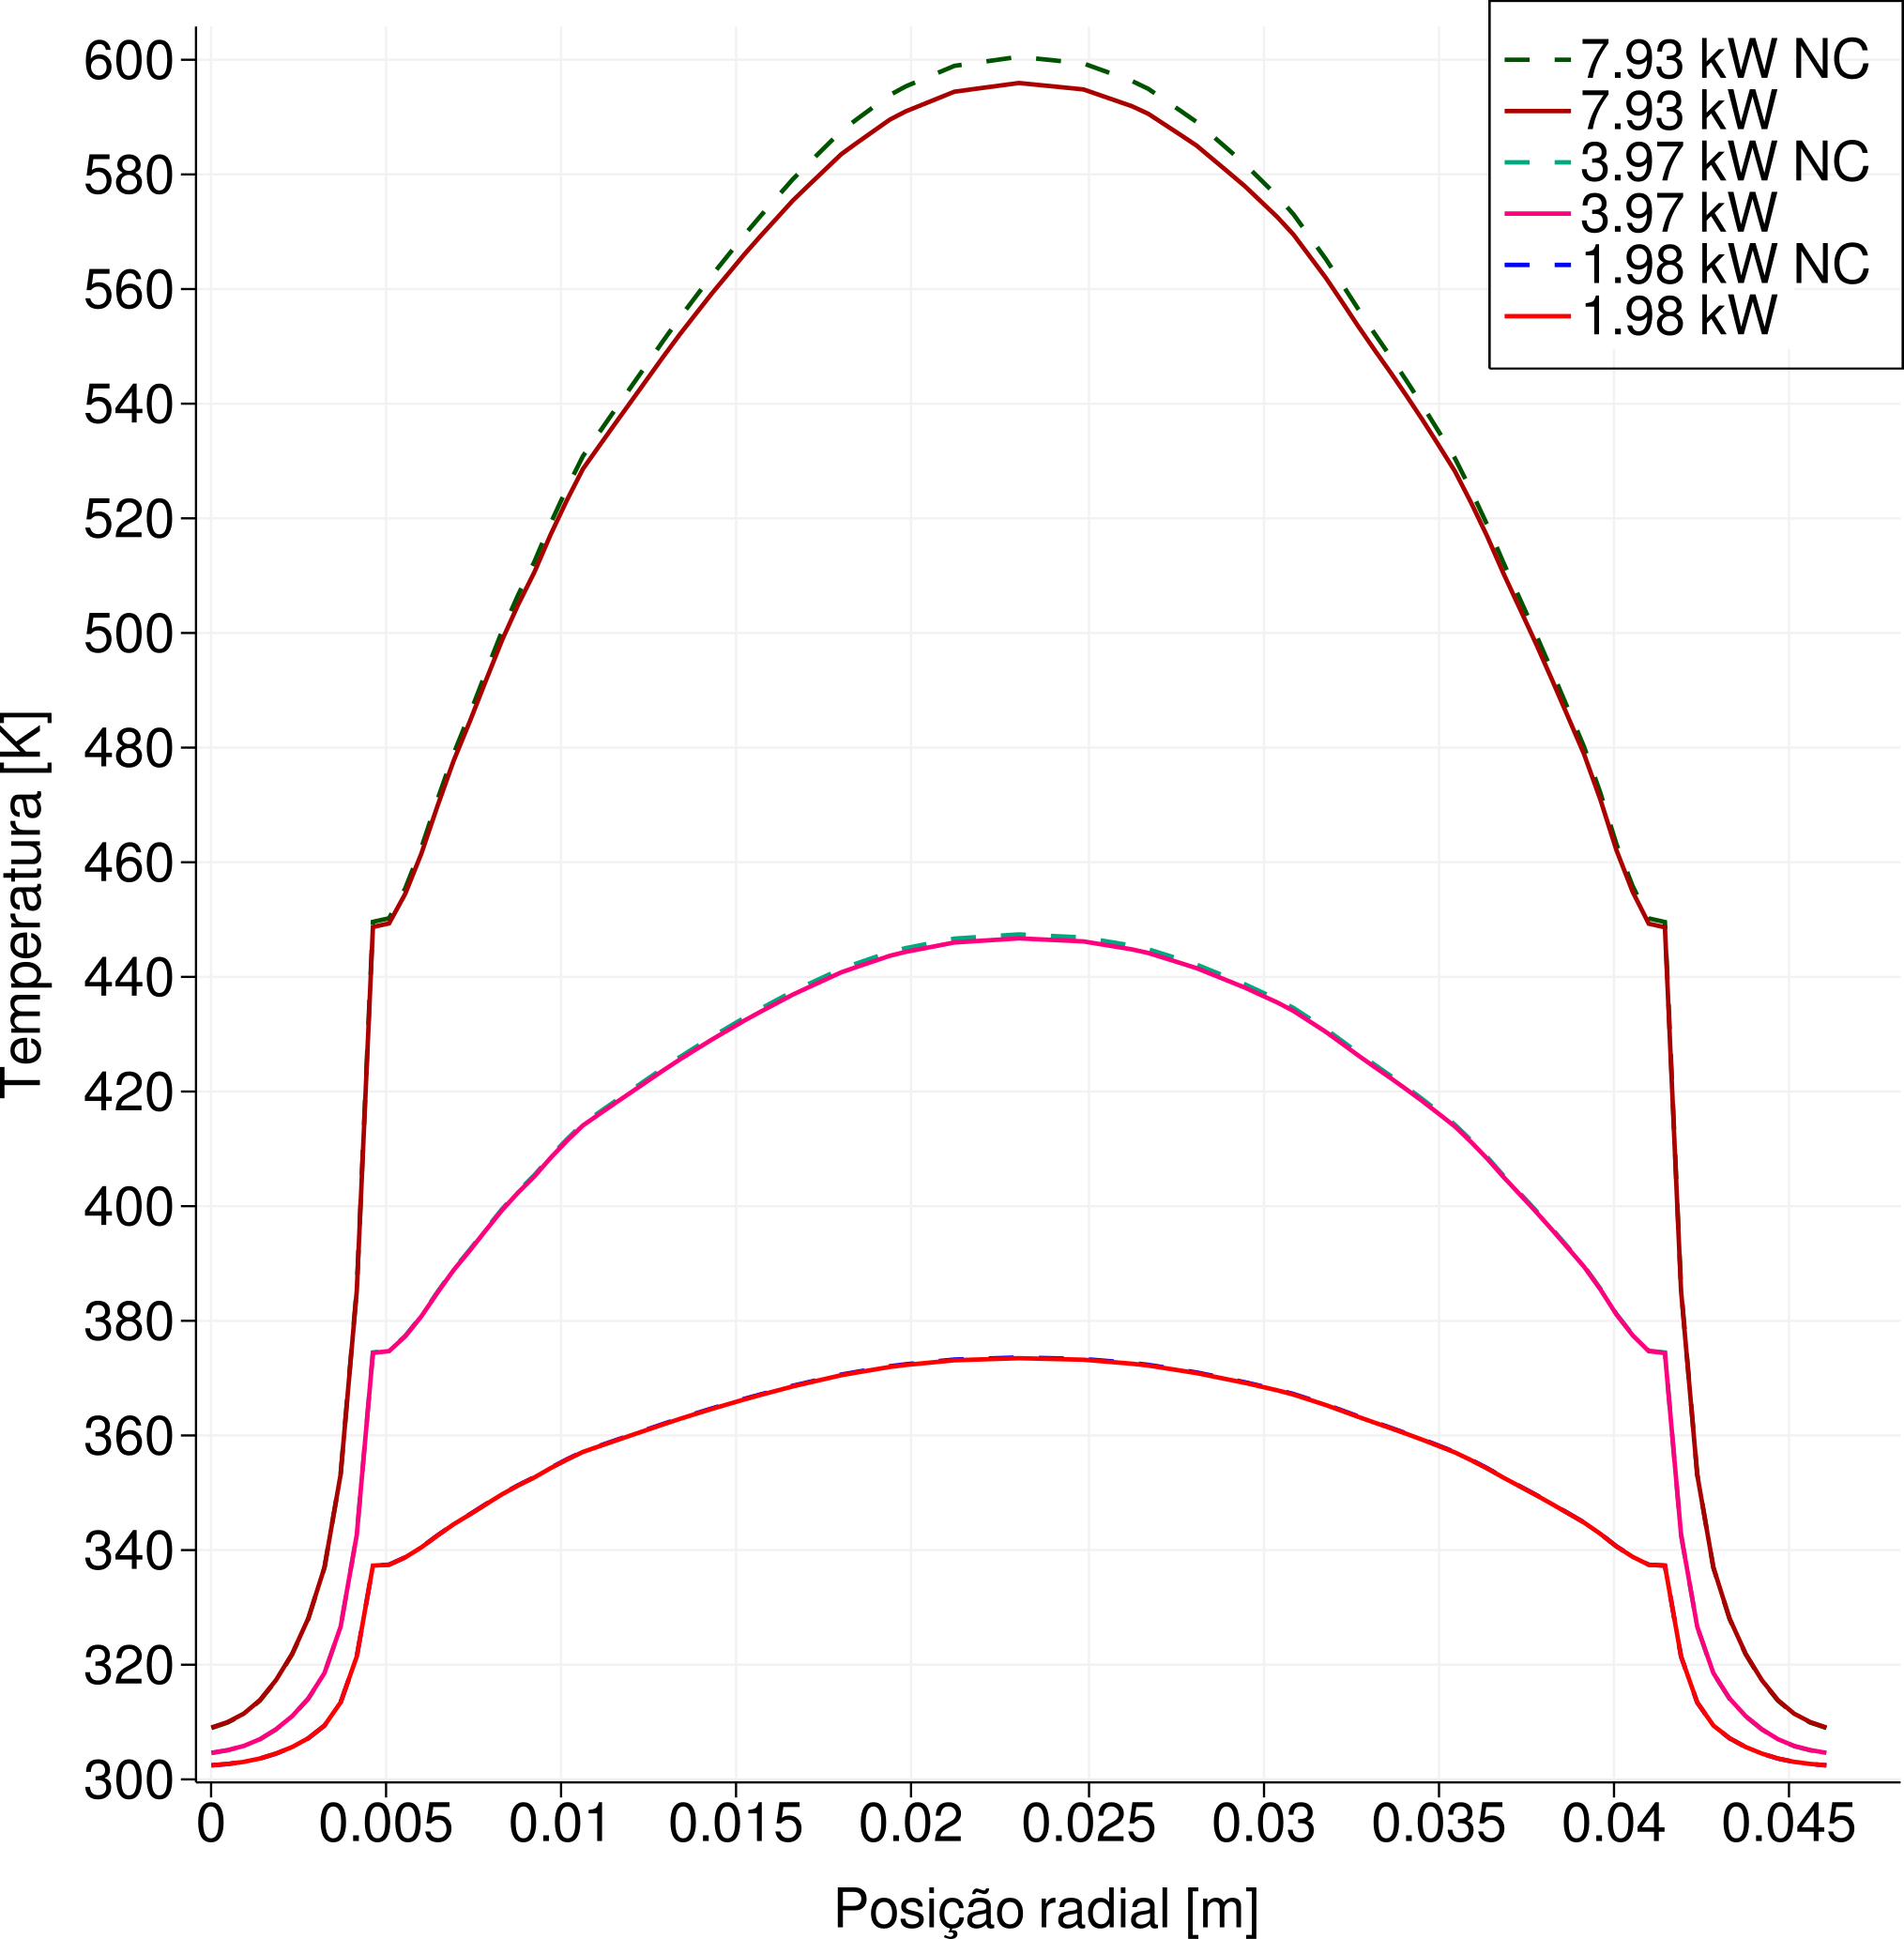
\includegraphics[width=\textwidth, height=7.0cm]{../figuras/T_x_all_square_port.png}
  \label{fig:keff50}
\end{frame}

%-------------------------------------------------
%\subsection{Gráficos}
\begin{frame}
  \frametitle{Resultados}
  \framesubtitle{Convergência}
  Variação dos fatores de multiplicação efetivo ($k_{eff}$).
  \centering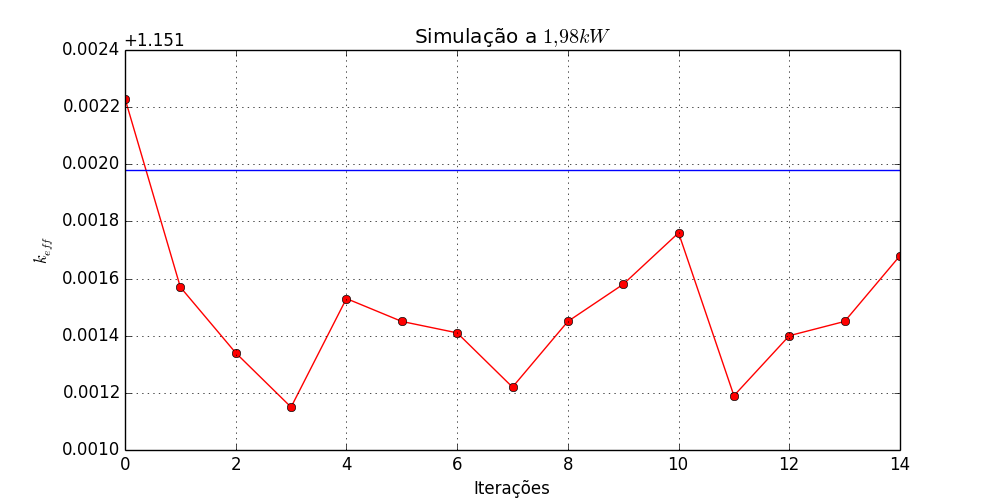
\includegraphics[scale=0.45]{../figuras/plot50.png}
  \label{fig:keff50}
\end{frame}

%-------------------------------------------------
\begin{frame}
  \frametitle{Resultados}
  \framesubtitle{Convergência}
  Variação dos fatores de multiplicação efetivo ($k_{eff}$).
  \centering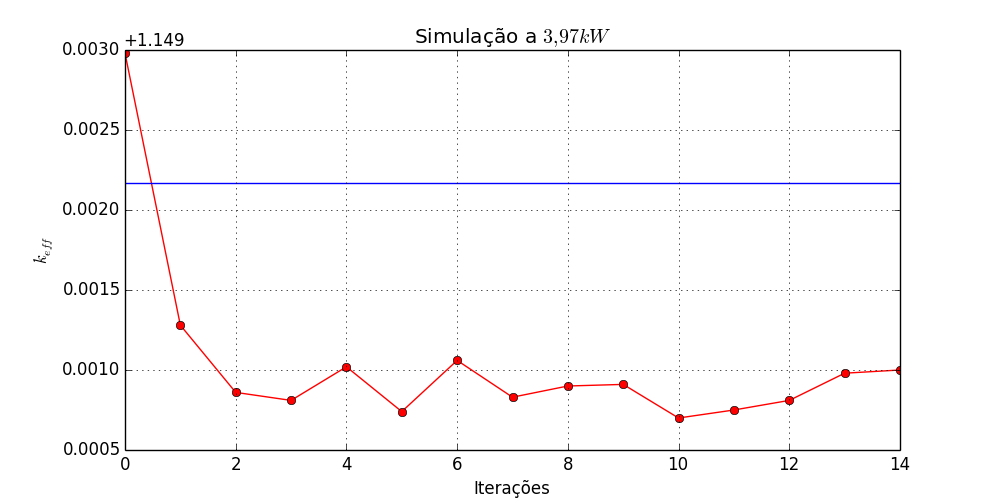
\includegraphics[scale=0.45]{../figuras/plot100.png}
  \label{fig:keff100}
\end{frame}

%-------------------------------------------------
\begin{frame}
  \frametitle{Resultados}
  \framesubtitle{Convergência}
  Variação dos fatores de multiplicação efetivo ($k_{eff}$).
  \centering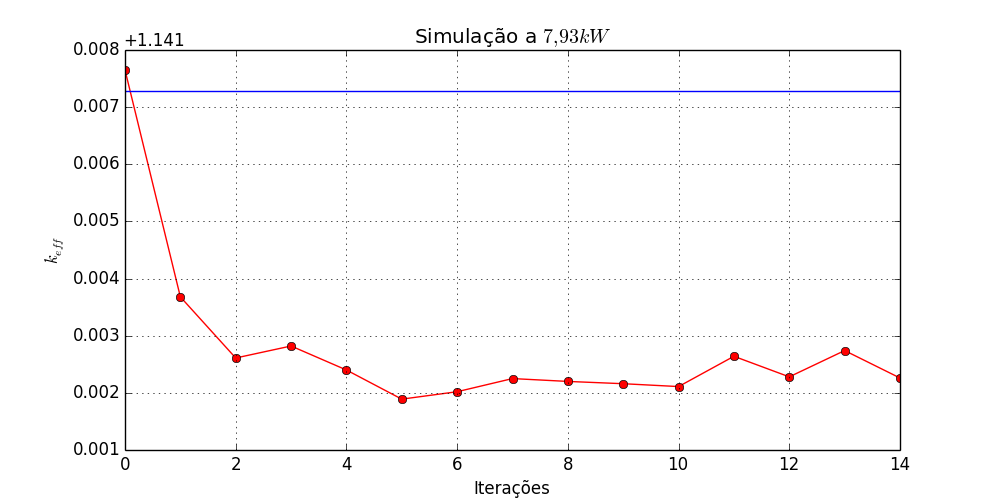
\includegraphics[scale=0.45]{../figuras/plot200.png}
  \label{fig:keff200}
\end{frame}




%-------------------------------------------------
\subsection{Fator de multiplicação}
\begin{frame}
  \frametitle{Resultados}
  \framesubtitle{Fator de multiplicação}
\begin{table}[]
\centering
%\caption{My caption}
\begin{tabular}{l|r|r|r|}
\cline{2-4}
\multicolumn{1}{c|}{}          & \multicolumn{3}{c|}{$k_{eff}$}                                                                                                                                              \\ \hline
\multicolumn{1}{|c|}{Potência} & \multicolumn{1}{c|}{Não acoplado} & \multicolumn{1}{c|}{\begin{tabular}[c]{@{}c@{}}Acoplado\\ (média durante \\os cálculos)\end{tabular}} & \multicolumn{1}{c|}{Desvio padrão} \\ \hline
\multicolumn{1}{|l|}{1,98 kW}  & 1,15298                           & 1,15249                                                                                             & 0,000257                           \\ \hline
\multicolumn{1}{|l|}{3,97 kW}  & 1,15117                           & 1,15004                                                                                             & 0,000538                           \\ \hline
\multicolumn{1}{|l|}{7,93 kW}  & 1,14829                           & 1,14378                                                                                             & 0,001367                           \\ \hline
\end{tabular}
\end{table}
\end{frame}

%-------------------------------------------------
\begin{frame}
  \frametitle{Resultados}
  \framesubtitle{Robustez(?)}
  Variação do fator de multiplicação efetivo ($k_{eff}$) com mudanças em parâmetros de convergência.
  \centering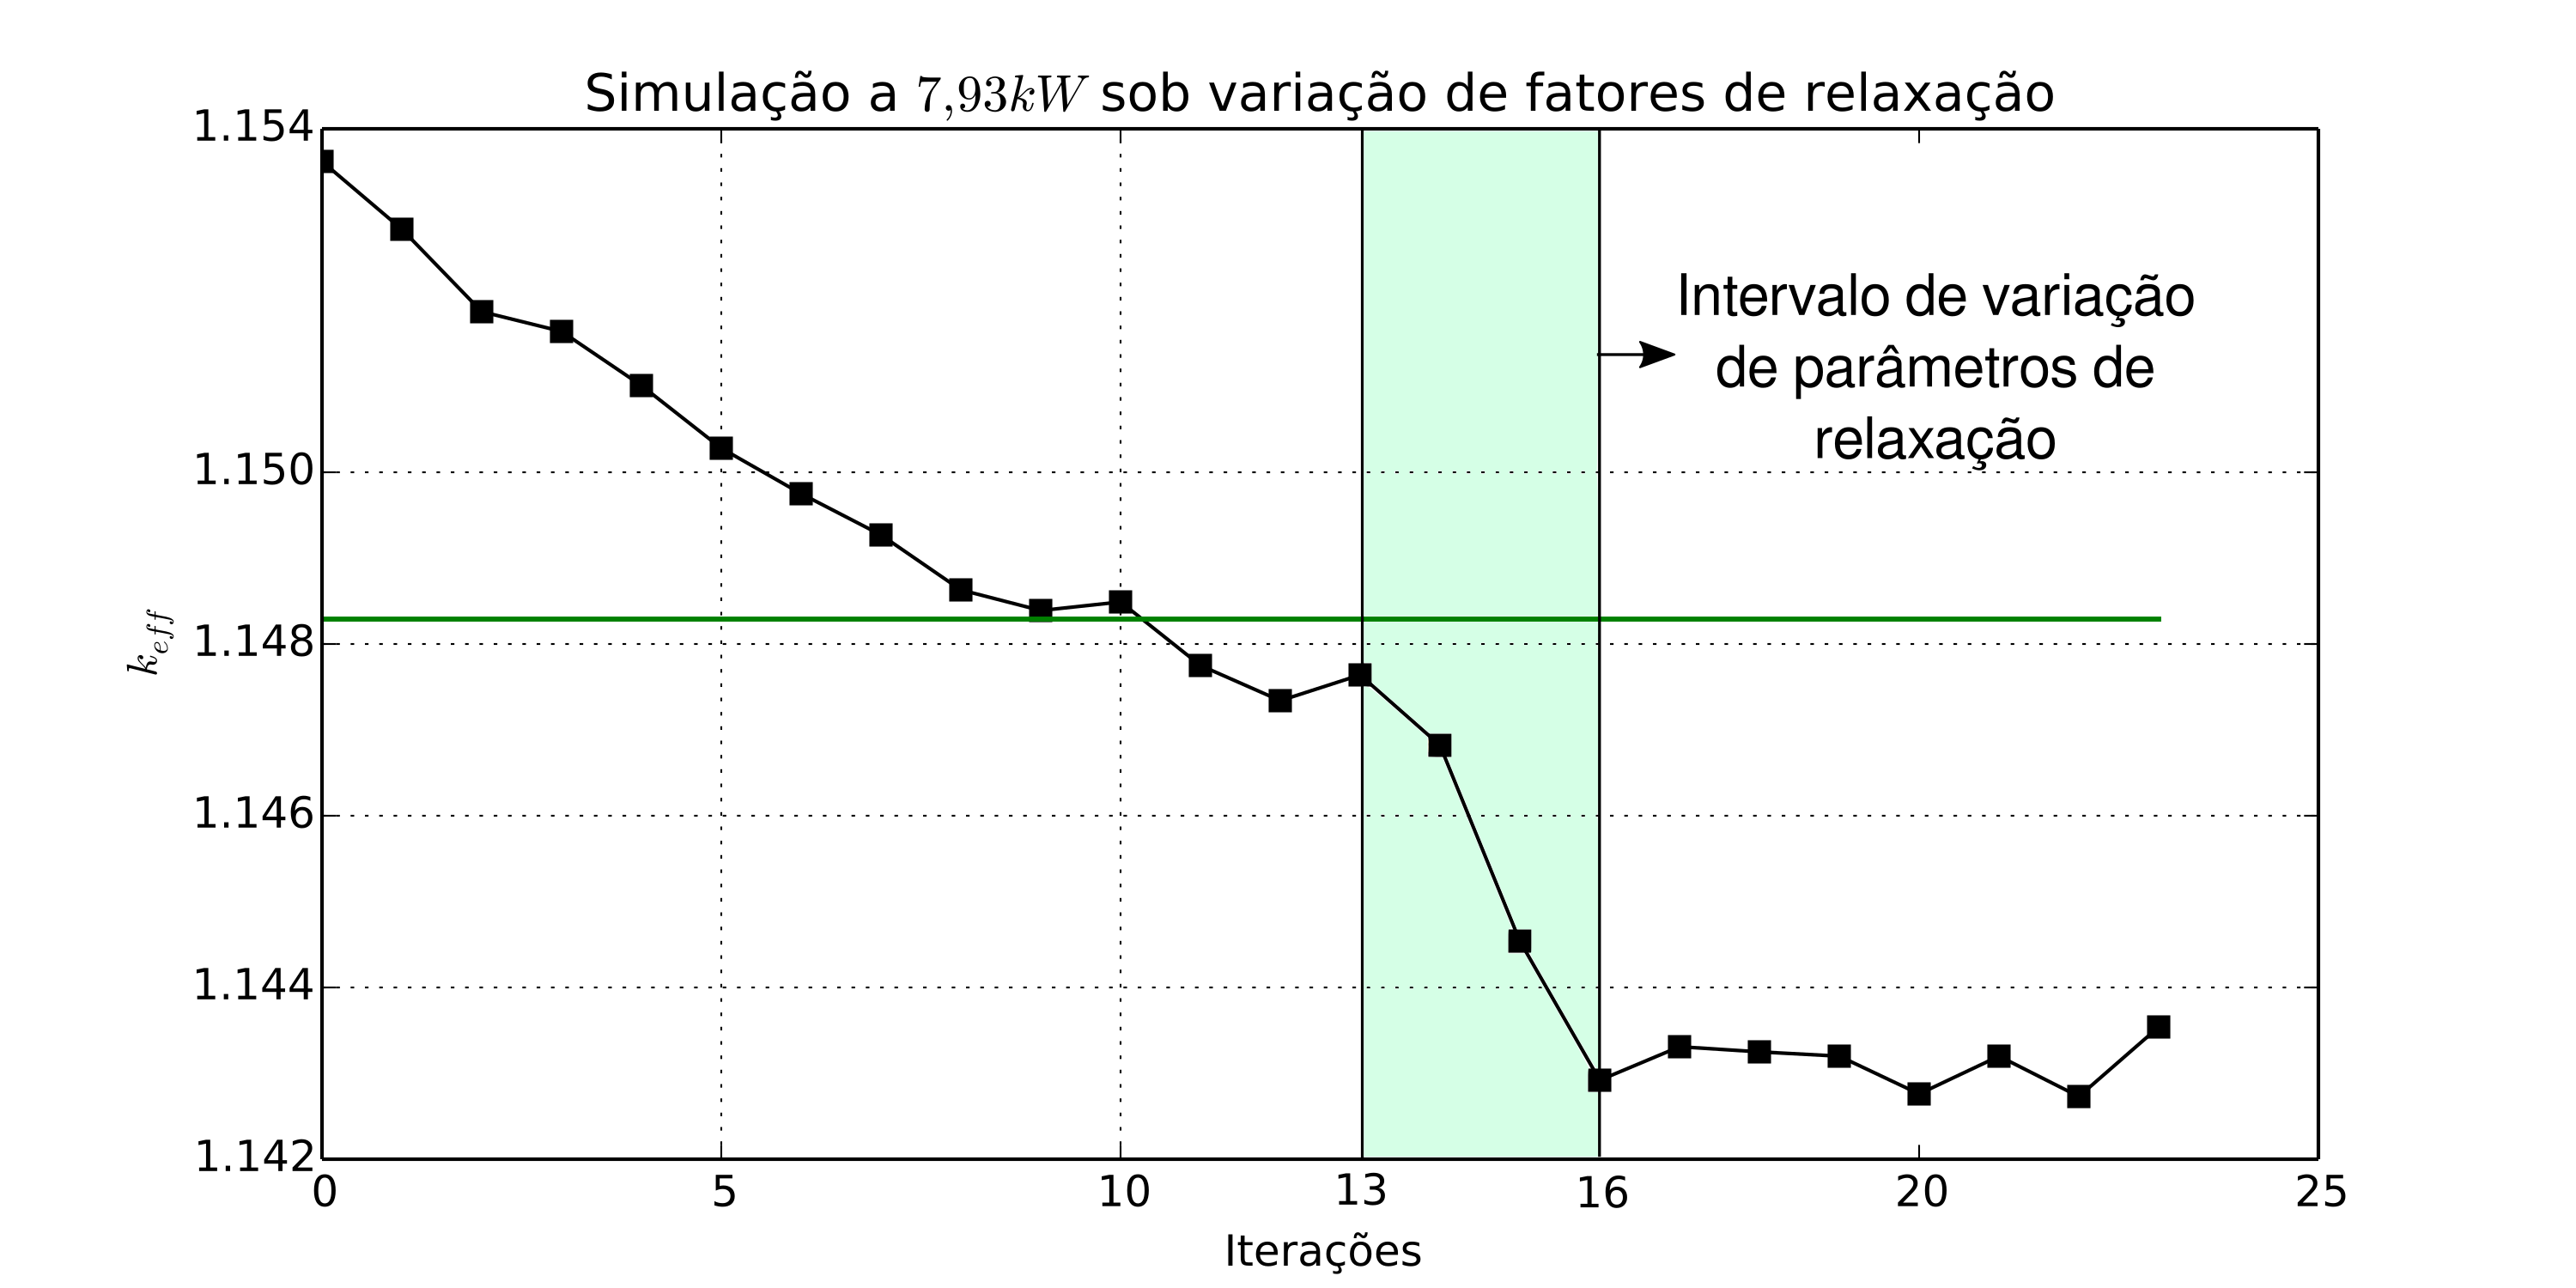
\includegraphics[scale=0.45]{../figuras/plot200-disturb-port.png}
  \label{fig:keff_dist}
%  \legend{Fonte: autor}
\end{frame}

\section{Conclusões}
%-------------------------------------------------
\begin{frame}
  \frametitle{Conclusões}
  \framesubtitle{}
\end{frame}

%-------------------------------------------------
\begin{frame}[allowframebreaks]
        \frametitle{Referências}
        \bibliographystyle{amsalpha}
        \bibliography{apre.bib}
\end{frame}


%-------------------------------------------------
% Frame escondido
\begin{frame}[noframenumbering]
  \frametitle{Respostas}
  \framesubtitle{Seções de choque}
  Teste
\end{frame}


\end{document}

